\documentclass[11pt,a4paper]{article}
\usepackage[T1]{fontenc}
\usepackage[utf8]{inputenc}
\usepackage{lmodern}
\usepackage{microtype}
\usepackage[margin=2.7cm]{geometry}
\usepackage{amsmath,amssymb,amsthm,mathtools}
\usepackage{booktabs,array,longtable}
\usepackage{xcolor}
\usepackage{tikz}
\usepackage{pgfplots}
\pgfplotsset{compat=1.18}
\usetikzlibrary{arrows.meta,calc,decorations.pathmorphing}
\usepackage[colorlinks=true,linkcolor=blue!55!black,citecolor=green!40!black,urlcolor=blue!55!black]{hyperref}
\usepackage[nameinlink,capitalize]{cleveref}
\usepackage{caption}
\captionsetup{font=small,labelfont=bf}

\numberwithin{equation}{section}
\theoremstyle{plain}
\newtheorem{proposition}{Proposition}[section]
\newtheorem{lemma}[proposition]{Lemma}
\theoremstyle{remark}
\newtheorem{remark}[proposition]{Remark}

% Symbols used throughout
\newcommand{\cN}{\mathcal{N}}
\newcommand{\cR}{\mathcal{R}}
\newcommand{\cQ}{\mathcal{Q}}
\newcommand{\cB}{\mathcal{B}}
\newcommand{\cI}{\mathcal{I}}
\newcommand{\cC}{\mathcal{C}}
\newcommand{\cT}{\mathcal{T}}
\newcommand{\sD}{\mathsf{D}}
\newcommand{\sM}{\mathsf{M}}
\newcommand{\sG}{\mathsf{G}}
\newcommand{\sP}{\mathsf{P}}
\newcommand{\sk}{\mathsf{k}}
\newcommand{\sgn}{\operatorname{sgn}}
\newcommand{\Res}{\operatorname*{Res}}
\newcommand{\ket}[1]{\langle #1\rangle}
\newcommand{\AdS}{\mathrm{AdS}}
\newcommand{\half}{\tfrac12}

\title{\vspace{-1.5cm}\textbf{\Large The melonic ladders of $\mathcal{N}=2$ SYK\\ as a half-supersymmetric Dirac problem in rigid AdS$_2$}}
\author{James Chryssanthacopoulos}
\date{\small Working draft, 6 November 2026}

\begin{document}
\maketitle

\begin{abstract}
\noindent
A recent construction of Thong shows that, once the centre of a conformal bilocal is integrated out, the ladder sum of a melonic CFT$_d$ is the Robin boundary-to-boundary propagator of one free scalar in rigid AdS$_{d+1}$. Here we work out the analogue for $\cN=2$ supersymmetric SYK at the charge-symmetric point. Zero total supermomentum removes every odd relative coordinate, and the $su(1,1|1)$ pair Casimir reduces to $L_0^2$, which derives the eigenvalue $H^2$ and the shadow $H\to-H$. The reduced kernel is a single boundary correlator of a Dirac field of mass $\mu=\half-1/q$ in AdS$_2$, with the ladder coupling entering as a constant boundary mass, and it reproduces the known kernels with no free constant. Integrating the full superconformal four-point function over the super-centre of a pair, instead of the centre, gives the same Dirac propagator, with one exponential per superblock. The neutral channels require two scalars with masses $\mu(\mu\mp1)$, which complete the Dirac field to a long AdS$_2$ multiplet. We show that the matrix boundary condition found in earlier work is the linear superfield condition $\Phi_+=c\,\Phi_-$ written on the cylinder, so its boundary term is a double-trace superpotential. This answers the question of how much bulk supersymmetry survives: at $g\neq0$ the boundary condition breaks $su(1,1|1)$, of dimension $4|4$, to $u(1|1)$, of dimension $2|2$, for either embedding of the algebra on the fields. Beyond Thong's two broken isometries, two of the four Killing supercharges are lost, and the two that remain close on a twisted Hamiltonian. We test these statements, together with the agreement of the construction with the published kernels, spectra and four-point data, by explicit computation. We also find that the Fock vacuum of the stationary quantization is invariant under the surviving charges only above a threshold $g_*<1$, and that the apparent mismatch at the $H=1$ multiplets is resolved by step-function terms in the family decomposition, supported on $\chi>1$.
\end{abstract}

\tableofcontents

\section{Introduction and summary}
\label{sec:intro}

In the usual large-$N$ dictionary, each single-trace primary corresponds to one bulk field. Melonic theories such as the SYK model~\cite{Maldacena:2016hyu,Kitaev} then seem to need an infinite tower of bulk fields, one for each bilinear family. Thong has shown that, at the level of the four-point function, one field is enough~\cite{Thong:2026}. Integrating out the centre of a bilocal turns the pair Casimir into an operator on a relative cylinder $\mathbb R\times S^{d-1}$, on which a family of dimension $h$ is represented by the energy $\omega=h-d/2$. The ladder sum is then the Robin boundary-to-boundary propagator of a single free scalar in rigid AdS$_{d+1}$. The constituent dimension fixes the mass, the ladder coupling fixes the Robin coefficient, and the Robin condition breaks $2d$ isometries, leaving $\mathbb R\times SO(d)$.

Thong remarks that supersymmetric SYK should go beyond a single scalar~\cite[p.~6]{Thong:2026}. This paper studies the $\cN=2$ model~\cite{Fu:2016vas}, whose ladders have been solved in components~\cite{Peng:2017spg} and in superspace~\cite{Bulycheva:2018qcp}. It has features absent from the cases Thong treats: constituents of different dimensions, mixed neutral channels, charged channels, kernels that aren't even in $h$, and two distinct protected multiplets. It also raises a natural question. If the bulk field content is supersymmetric, what happens to the supersymmetry when the boundary condition breaks the AdS isometries?

\subsection*{Main results}

\begin{enumerate}
\item \textbf{The cylinder (\cref{sec:cylinder}).} On a chiral--antichiral pair, zero total supermomentum leaves functions of the single invariant $x=\ket{12}$, so there is no odd relative coordinate. The $su(1,1|1)$ pair Casimir reduces to $L_0^2$, and $WCW^{-1}=\partial_\tau^2$. This derives the eigenvalue $H^2$ and shadow $-H$ of~\cite{Bulycheva:2018qcp}, and gives $\omega=H$.

\item \textbf{A Dirac response (\cref{sec:dirac}).} The reduced kernel is one boundary correlator of a dimension-$\delta$ fermion, with $\delta=1/q$, multiplied by a constant boundary vertex, \cref{eq:ladder-dirac}. Its eigenvalues reproduce the known kernels $k_A,k_S$ with no free constant.

\item \textbf{The full four-point function (\cref{subsec:supercentre}).} Integrating over the super-centre of a pair, its whole supertranslation orbit, turns the neutral superconformal four-point function into the same Dirac propagator, family by family. Each superblock gives the single exponential $e^{-H|\tau|}$, where the ordinary centre integral gives two. The trigonometric factors in the coefficients cancel, as in Thong's case, and the reduction holds at every $g$.

\item \textbf{The neutral channels (\cref{sec:neutral}).} An ordinary centre integral keeps all components of a multiplet, which is why a $2\times2$ matrix with frequency-dependent eigenvectors appears. We show that its resolvent is two Dirac resolvents, \cref{eq:ward}, and that the matrix boundary condition is the superfield condition $\Phi_+=c\,\Phi_-$ on the cylinder, \cref{eq:bc-super}, so the mixing matrix is derived rather than fitted.

\item \textbf{Broken supersymmetry (\cref{sec:susy}).} At $g\neq0$,
\begin{equation*}
su(1,1|1)\ \longrightarrow\ u(1|1),\qquad\text{dimension }4|4\to2|2.
\end{equation*}
The two broken bosonic generators are Thong's $E_\pm$. In addition, two of the four Killing supercharges are broken, in each of the two embeddings of the superalgebra on the fields. The two that survive close on the twisted Hamiltonian $L_0-\half J_0$, and on them the boundary data form ordinary superfields of flat $\cN=2$ quantum mechanics. The other two Killing spinors still give odd symmetries of the boundary condition, but only in the other embedding, and the four together do not close on a Lie superalgebra with constant structure constants.

\item \textbf{A BPS threshold (\cref{sec:stability}).} The Fock vacuum of the stationary quantization is invariant under the surviving charges only if $2\omega=2H-1\ge0$. This is saturated at the formal coupling $g_*<1$ where the lowest even-sector mode has zero frequency. Below $g_*$, that vacuum has energy $\half-H$ and isn't invariant, whereas a state with one Dirac mode filled is invariant and carries R-charge. The four-point function on $0<z<1$ stays smooth throughout.

\item \textbf{The exceptional multiplets (\cref{sec:fourpoint}).} Of the two $H=1$ multiplets, one is Thong's mechanism in $\cN=2$ form: an enhanced mode that the centre integral kills, leaving a finite remainder. The other is its mirror image. It has vanishing OPE coefficient on $0<\chi<1$ yet nonzero reduced weight, because the family is a finite step function supported on $\chi>1$.
\end{enumerate}

\Cref{tab:dictionary} compares the two constructions.

\begin{table}[t]
\centering
\renewcommand{\arraystretch}{1.25}
\begin{tabular}{@{}lll@{}}
\toprule
& Thong, SYK ($d=1$) & $\cN=2$ SYK (this paper)\\
\midrule
Reduced Casimir & $\partial_\tau^2-\tfrac14$ & $\partial_\tau^2$\\
Cylinder energy & $\omega=h-\half$ & $\Omega=H$\\
Cylinder weight & $a=2\Delta-\half$ & $a=2\Delta=\delta$\\
Bulk field & scalar, $m^2=\nu^2-\tfrac14$ & Dirac, $m_F=\mu$; scalars $\mu(\mu\mp1)$\\
Rung & Neumann propagator & Dirac boundary correlator\\
Ladder sum & Robin propagator & Dirac propagator with boundary mass\\
Boundary condition & $B=\kappa A$ & $b_F=g\sigma_pL_q\,a_F$; $\Phi_+=c\,\Phi_-$\\
Spectrum & $\cR_J(\omega)=\kappa$ & $\cR_{F,p}(\Omega)=g\sigma_pL_q$\\
Reduced family & $\cI(h)\,e^{-(h-\frac12)|\tau|}$ & $\cI_s(H)\,e^{-H|\tau|}$\\
Bulk symmetry at $g=0$ & $sl(2,\mathbb R)$ & $su(1,1|1)$\\
Bulk symmetry at $g\neq0$ & $\mathbb R$ & $u(1|1)$: $\mathbb R\times U(1)_R$, 2 supercharges\\
\bottomrule
\end{tabular}
\caption{Thong's construction at $d=1$ and its $\cN=2$ analogue. Here $\nu=d-2\Delta_\phi$ in the middle column, and $\nu=1-\delta$, $\mu=\half-\delta$, $\delta=1/q$ in the last. A reduced family is the centre integral of a block in the middle column, and the super-centre integral of a superblock in the last.}
\label{tab:dictionary}
\end{table}

\subsection*{Scope and status}

As in~\cite{Thong:2026}, this is a statement about four-point data at leading order in $1/N$, not an equivalence of theories. Multiparticle bulk states do not correspond to multi-trace operators, and we do not address higher-point functions or gravity. Derivations are at a physicist's level of rigour, and we don't prove convergence of the infinite family sums. Most closed-form statements below were tested numerically or symbolically, and the published formulas were transcribed and compared directly; \cref{app:checks} lists the tests, and the statements derived only by hand. We distinguish these from conjectures, which are flagged as such. As in~\cite{Thong:2026}, the reductions of families use a continuation of each family outside the region of its operator expansion, and we don't prove that they commute with the infinite sum over families (\cref{sec:discussion}).

Our starting point was an earlier unpublished note that proposed the matrix boundary condition and the reconstruction formula. Its formulas pass the tests listed here, and its central claims are given a derivation. We searched for prior work on the $\cN=2$ extension and found none, but the search was not exhaustive. The closest precedents for the boundary-condition analysis are Amsel--Marolf~\cite{Amsel:2008iz} and Correa et al.~\cite{Correa:2019rdk}; see \cref{subsec:compare}.

\section{The model and its ladders}
\label{sec:model}

\subsection{Two-point functions}

The model has $N$ complex fermions $\psi_i$ and auxiliary complex bosons $b_i$, with supercharge built from an odd number $q\ge3$ of fermions~\cite{Fu:2016vas}. We use the component conventions of~\cite{Peng:2017spg}, with
\begin{equation}
\ket{C_{i_1\cdots i_q}\bar C_{i_1\cdots i_q}}=\frac{(q-1)!\,J}{N^{q-1}}.
\end{equation}
In the conformal limit, at the charge-symmetric point,
\begin{equation}\label{eq:props}
G_\psi(\tau)=b_\psi\frac{\sgn\tau}{|\tau|^{\delta}},\qquad G_b(\tau)=-\partial_\tau G_\psi(\tau)=\frac{\delta\,b_\psi}{|\tau|^{1+\delta}},\qquad Jb_\psi^q=\frac{\tan(\pi\delta/2)}{2\pi},
\end{equation}
so the dimensions are $\Delta_\psi=\delta/2$ and $\Delta_b=(1+\delta)/2$. We will use throughout
\begin{equation}\label{eq:params}
\delta=\frac1q,\qquad\nu=1-\delta,\qquad\mu=\half-\delta,\qquad L_q=2(q-1)4^{-\nu},\qquad\sigma_p=(-1)^p.
\end{equation}
Note that $0<\mu<\half$ and $\half<\nu<1$. The label $p=0,1$ is the parity of the fermion-pair component under exchange. The relation $G_b=-\partial G_\psi$ is the zero-supermomentum relation of \cref{sec:cylinder} applied to the propagator.

In superspace~\cite{Fu:2016vas,Bulycheva:2018qcp}, the chiral field is $\Psi=\psi(\tau+\theta\bar\theta)+\theta b$, and correlators depend on the invariant
\begin{equation}\label{eq:bracket}
\ket{12}=\tau_{12}-2\bar\theta_1\theta_2-\theta_1\bar\theta_1-\theta_2\bar\theta_2,
\end{equation}
which is chiral in the first point and antichiral in the second. The superfield dimension satisfies $2\Delta=\delta$. The normalization of $b$ in~\cite{Bulycheva:2018qcp} differs from~\eqref{eq:props} by a factor of 2 in $G_b$, which accounts for $4\pi$ in place of $2\pi$ in the relation for $Jb^q$ there. Kernels are unaffected.

\subsection{Ladder kernels}

There are two kinds of ladder. The charged channel has $\psi b$ on one side and $\bar\psi\bar b$ on the other, with a diagonal kernel~\cite[(2.12)]{Peng:2017spg},
\begin{equation}\label{eq:Kd}
K^d(1,2;3,4)=J(q-1)\,G_\psi(\tau_{14})G_b(\tau_{23})G_\psi(\tau_{34})^{q-2}.
\end{equation}
The neutral channels $\psi\bar\psi$ and $b\bar b$ mix, through a matrix kernel with entries~\cite[(2.22)--(2.24)]{Peng:2017spg}
\begin{equation}\label{eq:Kmatrix}
\begin{aligned}
K^{11}&=J(q-1)(q-2)\,G_\psi(\tau_{14})G_\psi(\tau_{23})G_b(\tau_{34})G_\psi(\tau_{34})^{q-3},\\
K^{12}&=J(q-1)\,G_\psi(\tau_{14})G_\psi(\tau_{23})G_\psi(\tau_{34})^{q-2},\\
K^{21}&=J(q-1)\,G_b(\tau_{14})G_b(\tau_{23})G_\psi(\tau_{34})^{q-2},\qquad K^{22}=0,
\end{aligned}
\end{equation}
which is $K=C_0V$ with diagonal rails $C_0$. We write $g$ for a coupling multiplying each rung, with the physical theory at $g=1$. Its meaning at $g\neq1$ is discussed in \cref{subsec:line}.

Everything is controlled by two functions~\cite{Peng:2017spg,Bulycheva:2018qcp},
\begin{equation}\label{eq:kAkS}
k_{A,S}(H)=-C_\delta\,\Gamma(\delta-H)\Gamma(\delta+H)\,[\sin\pi\delta\mp\sin\pi H],\qquad C_\delta=\frac{\nu\Gamma(\nu)}{\pi\delta\Gamma(\delta)},
\end{equation}
which satisfy $k_A(H)=k_S(-H)$, $k_A(n)=k_S(n)$ at integers, $k_{A,S}(1)=1$ and $k_{A,S}(0)=-(q-1)$. In terms of them, the eigenvalues of the neutral kernel at component dimension $h$ are
\begin{equation}\label{eq:spectra}
\operatorname{spec}\sk_1(h)=\{k_A(h),\,k_S(h-1)\},\qquad\operatorname{spec}\sk_0(h)=\{k_S(h),\,k_A(h-1)\},
\end{equation}
and those of the charged kernel at dimension $h$ are $k_A(h-\half)$ and $k_S(h-\half)$. So each root of $gk_\alpha(H)=1$ gives a multiplet with component dimensions
\begin{equation}\label{eq:multiplet}
(H,\ H+\half,\ H+\half,\ H+1).
\end{equation}
At $q=3$, $g=1$, the first nonexceptional roots are $H_S=2.82114\ldots$ and $H_A=3.06590\ldots$, in agreement with the spectra of~\cite{Fu:2016vas,Peng:2017spg}.

We checked~\eqref{eq:kAkS}--\eqref{eq:spectra} against the printed formulas of~\cite{Peng:2017spg} entry by entry, and against~\cite{Fu:2016vas}. Our~\eqref{eq:kAkS} has the opposite overall sign to the literal~\cite[(4.48), (4.49)]{Bulycheva:2018qcp}. Those printed signs disagree with (4.51) together with (B.8) of the same paper, with~\cite{Peng:2017spg}, and with its statement that $k=1$ at $h=1$. \Cref{app:conventions} lists this and the other printed discrepancies we encountered.

\subsection{Two protected multiplets}

At $g=1$ both branches have a root at $H=1$, with component dimensions $(1,\tfrac32,\tfrac32,2)$. As anticipated in~\cite{Fu:2016vas} and confirmed in~\cite{Peng:2017spg}, they differ. The $S$-branch multiplet gives a divergence in the conformal ladder, and is expected to correspond to the super-Schwarzian. The $A$-branch multiplet gives no divergence, and is expected to correspond to operators of the IR theory associated with an extra symmetry of the low-energy equations~\cite[Sec.~VI]{Fu:2016vas}. We return to this in \cref{sec:fourpoint}.

\section{Zero supermomentum and the relative cylinder}
\label{sec:cylinder}

\subsection{The superconformal generators}

We use the $su(1,1|1)$ generators of~\cite[App.~A]{Bulycheva:2018qcp} acting on $(\tau,\theta,\bar\theta)$, for a field of dimension $\Delta$ and R-charge $Q$:
\begin{equation}\label{eq:generators}
\begin{aligned}
L_1&=-\partial_\tau,\qquad L_0=-\tau\partial_\tau-\half\theta\partial_\theta-\half\bar\theta\partial_{\bar\theta}-\Delta,\qquad J_0=-\theta\partial_\theta+\bar\theta\partial_{\bar\theta}+Q,\\
L_{-1}&=-\tau^2\partial_\tau-\tau\theta\partial_\theta-\tau\bar\theta\partial_{\bar\theta}-2\tau\Delta-Q\,\theta\bar\theta,\\
G_{-1/2}&=\partial_{\bar\theta}-\theta\partial_\tau,\qquad G_{+1/2}=\tau\partial_{\bar\theta}-\tau\theta\partial_\tau-(2\Delta+Q)\theta-\theta\bar\theta\partial_{\bar\theta},\\
\bar G_{-1/2}&=\partial_\theta-\bar\theta\partial_\tau,\qquad \bar G_{+1/2}=\tau\partial_\theta-\tau\bar\theta\partial_\tau-(2\Delta-Q)\bar\theta+\theta\bar\theta\partial_\theta.
\end{aligned}
\end{equation}
Three remarks are needed to use these. First, the printed normalization of the R-charge is inconsistent: the coefficient $Q/2$ printed in $L_{-1}$, $G_{+1/2}$ and $\bar G_{+1/2}$ doesn't close with the constant $Q$ in $J_0$. We repair this by $Q/2\to Q$ in those three generators, as in~\eqref{eq:generators}; the alternative, $Q\to Q/2$ in $J_0$, differs only in how $Q$ is normalized. Ours is the normalization of~\cite{Fu:2016vas}, in which the supercharge has R-charge 1. Second, the printed Casimir has $-L_1L_{-1}$, with the translation on the left, while its fermionic terms have translations on the right, and it isn't central. The central operator, with translations acting first in every term, is
\begin{equation}\label{eq:casimir}
C=L_0^2-\tfrac14J_0^2-L_{-1}L_1+\half\big(G_{+1/2}\bar G_{-1/2}+\bar G_{+1/2}G_{-1/2}\big).
\end{equation}
As evidence that this ordering is what was intended, it reproduces the printed one-particle values~\cite[(A.10)--(A.12)]{Bulycheva:2018qcp} exactly when combined with the printed generators. Those values aren't constant on the multiplet, as a central element must be. With the closed algebra, $C=\Delta^2-Q^2/4$ on all components. None of this affects results at zero total charge. Third, $Q=0$ holds only for the pair. The two-point function $\ket{12}^{-2\Delta}$ is annihilated by all total generators only for $Q_1=-2\Delta$, $Q_2=+2\Delta$, in the normalization of~\eqref{eq:generators}, which is the chiral-primary condition of~\cite{Fu:2016vas}. With these corrections, a direct implementation on the Grassmann algebra reproduces the cross-ratio form of the Casimir~\cite[(4.9), (A.16)]{Bulycheva:2018qcp},
\begin{equation}\label{eq:casimir-chi}
\cC=\chi^2(1-\chi)\partial_\chi^2+\chi(1-\chi)\partial_\chi,
\end{equation}
on all odd components, with $\chi=\ket{12}\ket{34}/(\ket{14}\ket{32})$.

\subsection{Reduction}

Thong's first step is to restrict the pair Casimir to zero total momentum. The supersymmetric analogue is immediate.

\begin{proposition}\label{prop:cylinder}
Let $f$ be a function on a chiral--antichiral pair annihilated by the total $L_1$, $G_{-1/2}$ and $\bar G_{-1/2}$. Then $f=f(x)$ with $x=\ket{12}$, and
\begin{equation}\label{eq:reduced-casimir}
C\,f(x)=L_0^2f(x),\qquad L_0f(x)=-(x\partial_x+2\Delta)f(x).
\end{equation}
With $x=e^\tau n$, $n=\pm1$, and $(Wf)(\tau,n)=e^{2\Delta\tau}f(e^\tau n)$,
\begin{equation}\label{eq:WCW}
WCW^{-1}=\partial_\tau^2.
\end{equation}
\end{proposition}

\begin{proof}
Chirality leaves the coordinates $(\tau_1,\bar\theta_1;\tau_2,\theta_2)$, which is $2|2$. The three conditions remove $1|2$, leaving $1|0$, and $\ket{12}$ is the unique invariant~\cite{Bulycheva:2018qcp}. Each term of~\eqref{eq:casimir} other than $L_0^2$ and $J_0^2$ has a translation on the right, so it annihilates $f$. Also $J_0f=0$, since $\bar\theta_1\theta_2$ is neutral and $Q_1+Q_2=0$. Finally $\ket{12}$ has weight $-1$, which gives the action of $L_0$, and $W$ turns $-(x\partial_x+2\Delta)$ into $-\partial_\tau$.
\end{proof}

So \emph{the relative space has no odd directions}: the cylinder is the ordinary $\mathbb R\times S^0$, with $S^0=\{\pm1\}$. On $e^{H\tau}Y_p(n)$, with $Y_p$ of parity $\sigma_p$, the eigenvalue is $H^2$, so $\Omega=H$ and the shadow is $-H$. This derives what~\cite{Bulycheva:2018qcp} finds by computing~\eqref{eq:casimir-chi} directly.

The difference from Thong is a single term. Reordering in the same way gives $L_0^2+(1-\cN/2)L_0$ for $\cN=0,1,2$ at zero (super)momentum. With $L_0\to-h$ this is
\begin{equation}\label{eq:pattern}
h(h-d_s),\qquad d_s=1-\frac{\cN}{2},\qquad\omega=h-\frac{d_s}{2},
\end{equation}
which matches the eigenvalues $h(h-1)$~\cite{Maldacena:2016hyu}, $h(h-\half)$~\cite{Murugan:2017eto} and $h^2$~\cite{Bulycheva:2018qcp}. We also confirmed the $\cN=1$ case directly from the generators of~\cite{Murugan:2017eto}, on functions of $t_{12}-\theta_1\theta_2$. The number $d_s$ is the scaling weight of the measure on the superline with $\cN$ real odd coordinates: $d\tau\,d^{\cN}\theta$ scales with weight $-(1-\cN/2)$. So $\cN=2$ has a dimensionless measure, which is why the Casimir has no linear term. $\cN=2$ is special in another way. For $\cN=1$, the pair coordinates are $2|2$, supertranslations remove only $1|1$, and an odd relative coordinate remains. So $\cN=1$ has a true super-cylinder, and it isn't simply a smaller version of this problem.

\subsection{Components}

Expanding~\eqref{eq:bracket},
\begin{equation}\label{eq:component-relation}
f(\ket{12})=f(\tau_{12})-2\bar\theta_1\theta_2f'(\tau_{12})+\cdots,
\end{equation}
so at zero supermomentum the $b\bar b$ entry of a neutral bilocal is a derivative of the $\psi\bar\psi$ entry. In the normalization of~\eqref{eq:props} this reads $f_b=-\partial_\tau f_\psi$. The $h=0$ case is~\eqref{eq:props} itself. As a test, the matrix kernels of~\cite{Peng:2017spg} know nothing about superspace, but act on the two-component functions $(\sgn\tau\,|\tau|^{h-\delta},\ c\,|\tau|^{h-\delta-1})$ and their even partners, and on the branch $k_A$ (odd sector) or $k_S$ (even sector) their right eigenvector has exactly
\begin{equation}\label{eq:eigvec-bottom}
c=-(h-\delta)
\end{equation}
for all $h$ and $q$ tested, which is~\eqref{eq:component-relation}. The other branch has
\begin{equation}\label{eq:eigvec-top}
c=h+\delta-1,
\end{equation}
which isn't a function of $\ket{12}$ alone.

This explains the structure of the neutral problem. An ordinary centre integral imposes only $L_1=0$, and functions annihilated by $L_1$ but not by $G_{-1/2},\bar G_{-1/2}$ are still allowed. So it keeps both the bottom and the top components of each multiplet: two branches, and a matrix. Superspace keeps one function $f(x)$, one branch per parity, and one scalar kernel. We now compute that kernel.

\section{The reduced ladder is a Dirac response}
\label{sec:dirac}

\subsection{The reduced kernel}

Take the charged ladder with seed $F_0=G_\psi(\tau_{13})G_b(\tau_{24})$ and kernel~\eqref{eq:Kd}. Write $x=\tau_{12}$, $y=\tau_{34}$, and let $Y$ be the difference of the pair centres. As in~\cite{Thong:2026}, translation invariance gives fibrewise composition, $(KF)^{(0)}=K^{(0)}F^{(0)}$, on a common regulated domain.

\paragraph{The rail.} The chain integral~\cite[(C.3)]{Thong:2026}, with $2\Delta=\delta$, gives
\begin{equation}\label{eq:chain}
\int dz\,G_\psi(z)G_\psi(z-t)=b_\psi^2\,\mathbf C\,|t|^{2\mu},\qquad\mathbf C=2B(\nu,2\delta-1)-B(\nu,\nu).
\end{equation}
The first Beta function is defined by continuation, as the integral diverges in the infrared for $q\ge3$. Using $G_b=-\partial G_\psi$, the mixed rail is its derivative,
\begin{equation}\label{eq:rail}
\rho(t)\equiv\int dz\,G_\psi(z)G_b(z-t)=\rho_0\,\sgn(t)\,|t|^{-2\delta},\qquad\rho_0=2\mu\,b_\psi^2\,\mathbf C,
\end{equation}
which defines the short-distance divergence of the boson rail by the same continuation. Notice that the odd statistics of the rail are automatic: $\rho$ is odd, even though one of the two propagators is even.

\paragraph{Seed and rung.} In the seed $\tau_{13}-\tau_{24}=x-y$, while in the kernel $\tau_{14}-\tau_{23}=x+y$. Since $q-2$ is odd and $\delta(q-2)=2\mu$,
\begin{equation}\label{eq:reduced}
F_0^{(0)}(x,y)=\rho(x-y),\qquad K^{(0)}(x,y)=\rho(x+y)\,\mathcal V(y),\qquad\mathcal V(y)=v\,\sgn(y)\,|y|^{-2\mu},
\end{equation}
with $v=(q-1)Jb_\psi^{q-2}$. The appearance of $x+y$ is not an accident of labelling. The vertex exchanges which rail carries the fermion, and this makes the rung act with a reflection $y\to-y$.

\paragraph{The neutral channels see the same kernel.} Reduce the matrix kernel~\eqref{eq:Kmatrix} on a pair of the form $(f,-\partial f)$, which is~\eqref{eq:component-relation} in the present normalization. Its rails give $\int G_\psi G_\psi=b_\psi^2\mathbf C|x+y|^{2\mu}\equiv\mathcal A(x+y)$, with $\mathcal A'=\rho$, and $\int G_bG_b=-\rho'$. Since $(q-2)G_bG_\psi^{q-3}=-\partial G_\psi^{q-2}$, the first row is
\begin{equation}
\begin{aligned}
J(q-1)\int dy\,\mathcal A(x+y)\Big[-\partial_y\big(G_\psi^{q-2}\big)f-G_\psi^{q-2}\partial_yf\Big]&=J(q-1)\int dy\,\rho(x+y)\,G_\psi(y)^{q-2}f(y)\\
&=(K^{(0)}f)(x),
\end{aligned}
\end{equation}
after integrating by parts, and the second row is
\begin{equation}
J(q-1)\int dy\,\big(-\rho'(x+y)\big)G_\psi(y)^{q-2}f(y)=-\partial_x(K^{(0)}f)(x).
\end{equation}
So the subspace $\{(f,-\partial f)\}$ is invariant, and on it the $2\times2$ neutral kernel acts as the single scalar kernel $K^{(0)}$ of the charged channel. We checked the first row by direct quadrature on smooth test functions, and $\int G_bG_b=-\rho'$ from the chain formula. Superspace appears to explain why, though this step we did only by hand: with the odd coordinates of the outer points set to zero, the Grassmann integral in~\cite[(4.42)]{Bulycheva:2018qcp} acts on the rung and $f$ as a derivative, and its factor of 2 is compensated by the normalization noted in \cref{sec:model}. \Cref{subsec:supercentre} carries out the superspace version for the full four-point function.

\paragraph{The cylinder.} Set $x=e^\tau n$, $y=e^{\tau'}n'$. Then $|x\mp y|^2=e^{\tau+\tau'}[2\cosh(\tau-\tau')\mp2nn']$, and the powers of $|y|$ from the measure, the rung and the weight combine as $1-2\mu-\delta=\delta$. This is the analogue of Thong's cancellation, and it leaves
\begin{equation}\label{eq:S-kernel}
v(|x||y|)^\delta\rho(x-y)=c\,\mathfrak S(\tau-\tau';n,n'),\qquad c=v\rho_0,
\end{equation}
with
\begin{equation}\label{eq:S}
\mathfrak S(t;n,n)=n\frac{\sgn t}{|2\sinh\frac t2|^{2\delta}},\qquad\mathfrak S(t;n,-n)=\frac{n}{(2\cosh\frac t2)^{2\delta}}.
\end{equation}
These are the same-boundary and cross-boundary correlators of a fermionic operator of dimension $\delta$ on the two boundaries of the AdS$_2$ strip, which we identify in \cref{subsec:dirac-field}. The constant is
\begin{equation}\label{eq:c}
c=(q-1)Jb_\psi^q\,2\mu\,\mathbf C=-\frac{\nu\Gamma(\nu)}{2\delta\,\Gamma(\delta)\cos(\pi\delta)\,\Gamma(1-2\delta)}.
\end{equation}

On $g(\tau,n)=g_p(\tau)Y_p(n)$ the cylinder kernel preserves parity, and acts by convolution with
\begin{equation}\label{eq:kp-position}
\mathbf k_p(t)=c\left[\frac{1}{(2\cosh\frac t2)^{2\delta}}-\sigma_p\frac{\sgn t}{|2\sinh\frac t2|^{2\delta}}\right].
\end{equation}
Define, for $|\mathrm{Re}\,H|<\delta$,
\begin{equation}\label{eq:AB}
\begin{aligned}
A(H)&=\int dt\,\frac{e^{Ht}}{(2\cosh\frac t2)^{2\delta}}=\frac{\Gamma(\delta-H)\Gamma(\delta+H)}{\Gamma(2\delta)},\\
B(H)&=\int dt\,\frac{e^{Ht}\sgn t}{|2\sinh\frac t2|^{2\delta}}=\frac{2\cos(\pi\delta)\,\Gamma(1-2\delta)}{\pi}\Gamma(\delta-H)\Gamma(\delta+H)\sin\pi H,
\end{aligned}
\end{equation}
and note that $1/\Gamma(2\delta)=2\sin(\pi\delta)\cos(\pi\delta)\Gamma(1-2\delta)/\pi$. So
\begin{equation}\label{eq:AplusB}
A(H)+\sigma_pB(H)=\frac{2\cos(\pi\delta)\,\Gamma(1-2\delta)}{\pi}\,\Gamma(\delta-H)\Gamma(\delta+H)\,[\sin\pi\delta+\sigma_p\sin\pi H].
\end{equation}

\begin{proposition}\label{prop:kernel}
On $e^{H\tau}Y_p(n)$, continued meromorphically from the strip $|\mathrm{Re}\,H|<\delta$, the reduced kernel has eigenvalue
\begin{equation}\label{eq:kp}
c\,[A(H)+\sigma_pB(H)]=
\begin{cases}k_A(H),&p=1,\\ k_S(H),&p=0,\end{cases}
\end{equation}
with $k_A,k_S$ the functions~\eqref{eq:kAkS}. There is no free constant.
\end{proposition}

The mode $e^{H\tau}$ corresponds to the bilocal $|x|^{H-\delta}$, which is the three-point structure with the third operator at infinity, and $e^{-H\tau}$ is its shadow. Since $A$ is even and $B$ is odd, the shadow exchanges $k_A$ and $k_S$. This is the statement $k_A(H)=k_S(-H)$, which on the cylinder is $\tau\to-\tau$. We checked~\eqref{eq:AB} by direct integration, and~\eqref{eq:c},~\eqref{eq:kp} to working precision.

\subsection{The Dirac field}
\label{subsec:dirac-field}

Consider global AdS$_2$, $ds^2=\sec^2\theta\,(-dt^2+d\theta^2)$, with $\theta\in(-\frac\pi2,\frac\pi2)$ and $\zeta=\cos\theta$, and a Dirac field of mass $\mu$. With frames $\gamma^0=i\sigma_1$, $\gamma^1=-\sigma_3$ and $\Psi=\zeta^{1/2}\psi$, the equation $(\gamma^a\nabla_a-\mu)\Psi=0$ becomes
\begin{equation}\label{eq:HD}
i\partial_t\psi=H_D\psi,\qquad H_D=J_2\partial_\theta+\mu\sec\theta\,\sigma_1,\qquad J_2=\begin{pmatrix}0&-1\\1&0\end{pmatrix}.
\end{equation}
On a mode $e^{-i\Omega t}$, the rotation $\psi=e^{(\pi/4-\theta/2)J_2}(u,v)^T$ gives the first-order system
\begin{equation}\label{eq:first-order}
(\partial_\theta+\mu\tan\theta)u=(\omega+\mu)v,\qquad(-\partial_\theta+\mu\tan\theta)v=(\omega-\mu)u,\qquad\omega=\Omega-\half.
\end{equation}
At the right endpoint, $v\to a_F\zeta^{-\mu}$ and $u\to b_F\zeta^{\mu}$, so $a_F$ has weight $\half-\mu=\delta$ and $b_F$ has weight $\half+\mu=\nu$. If $v$ has parity $p$, then $u$ has parity $1-p$. Since $|\mu|<\half$ both falloffs are normalizable, and any relation between $a_F$ and $b_F$ compatible with the boundary form is allowed.

The regular solution of parity $p$ fixes the response~\cite{Thong:2026},
\begin{equation}\label{eq:RF}
\cR_{F,p}(\Omega)\equiv\frac{b_F}{a_F}=\frac{2\nu\,\cR_{\nu,p}(\Omega-\half)}{\Omega-\nu},\qquad\cR_{\rho,p}(\omega)=\frac{\Gamma(-\rho)}{\Gamma(\rho)}\prod_\pm\frac{\Gamma\big(\frac{p+\frac12+\rho\pm\omega}{2}\big)}{\Gamma\big(\frac{p+\frac12-\rho\pm\omega}{2}\big)}.
\end{equation}

\begin{proposition}\label{prop:response}
The response~\eqref{eq:RF} is the Fourier transform of the correlators~\eqref{eq:S}:
\begin{equation}\label{eq:RF-AB}
\frac{1}{\cR_{F,p}(H)}=-\mathfrak c\,[\sigma_pA(H)+B(H)],\qquad\mathfrak c=\frac{\Gamma(\delta+\half)}{\sqrt\pi\,\Gamma(\delta)}.
\end{equation}
Moreover $c=-L_q\mathfrak c$, so that
\begin{equation}\label{eq:k-RF}
k_p(H)=\frac{\sigma_pL_q}{\cR_{F,p}(H)},\qquad(p,\alpha)=(1,A),\ (0,S).
\end{equation}
\end{proposition}

Hence the seed is the free boundary correlator. Let $\mathfrak G_F=\mathfrak c\,\mathfrak S$, and let $(\mathsf R h)(\tau,n)=n\,h(\tau,-n)$, so that $\mathsf R^2=-1$. Then~\eqref{eq:reduced} and~\eqref{eq:S-kernel} say
\begin{equation}\label{eq:K-G}
WK^{(0)}W^{-1}=L_q\,\mathfrak G_F\,\mathsf R,\qquad v(|x||y|)^\delta F_0^{(0)}(x,y)=-L_q\,\mathfrak G_F(\tau-\tau';n,n').
\end{equation}
The structure is $K=C_0V$ with the constant boundary vertex $L_q\mathsf R$.

\subsection{The ladder}

Summing the geometric series, and continuing as a resolvent as in~\cite{Thong:2026},
\begin{equation}\label{eq:ladder-position}
v(|x||y|)^\delta F_g^{(0)}(x,y)=-L_q\,\mathfrak G_{F,g}(\tau-\tau';n,n'),\qquad\mathfrak G_{F,g}=\big(\mathfrak G_F^{-1}-gL_q\mathsf R\big)^{-1}.
\end{equation}
This is the $\cN=2$ analogue of~\cite[(3.11)]{Thong:2026}. No commutation of the rail and the vertex is assumed. A source $j$ for $b_F$ gives $b_F-gL_q\mathsf Ra_F=j$, so the source-free boundary condition is
\begin{equation}\label{eq:bc-dirac}
b_F=gL_q\mathsf R\,a_F,\qquad\text{i.e.}\qquad b_F=g\sigma_pL_q\,a_F\ \ \text{on parity }p,
\end{equation}
at the right endpoint. In the eigenbasis,
\begin{equation}\label{eq:ladder-dirac}
\boxed{\ \frac{k_p(H)}{1-gk_p(H)}=\sigma_pL_q\,G^F_{g,p}(H),\qquad G^F_{g,p}(\Omega)=\frac{1}{\cR_{F,p}(\Omega)-g\sigma_pL_q}.\ }
\end{equation}
So the operator spectrum is the normal-mode spectrum, $\cR_{F,p}(\Omega)=g\sigma_pL_q$, with $\Omega=H$.

\paragraph{The boundary vertex couples antipodal endpoints.} In terms of endpoint data, $a_F(-)=\sigma_pa_F(+)$ and $b_F(-)=-\sigma_pb_F(+)$, so~\eqref{eq:bc-dirac} reads $b_F(n)=n\,gL_q\,a_F(-n)$: the coupling connects the two boundaries of the strip. It is the $x+y$ of the rail that does this. See \cref{fig:strip}.

\paragraph{Spectral positivity.} The boundary form $\bar a_{F,1}b_{F,2}-\bar b_{F,1}a_{F,2}$ vanishes on~\eqref{eq:bc-dirac}, so $H_D$ is self-adjoint on it for real $g$. Thus
\begin{equation}\label{eq:spectral}
G^F_{g,p}(\Omega)=\sum_n\frac{w_n}{\Omega-\Omega_n},\qquad w_n=\frac{1}{\cR_{F,p}'(\Omega_n)}>0.
\end{equation}
The roots come in pairs: $\Omega_n$ at parity $p$ and $-\Omega_n$ at parity $1-p$, from $k_A(H)=k_S(-H)$. We confirmed $w_n>0$ at all roots with $|\Omega|<3.3$, for $q=3,5,7$ and $g=0.6,0.95$.

Unlike the scalars of the next section, the Dirac field has no difficulty with stationarity at any $g\in(0,1]$. Its boundary weight is $\delta>0$, and its correlators~\eqref{eq:S} decay. The failure of Thong's condition $a+J>0$ found for the $p=0$ neutral sector is entirely a feature of the bosonic components (\cref{sec:stability}).

\begin{figure}[t]
\centering
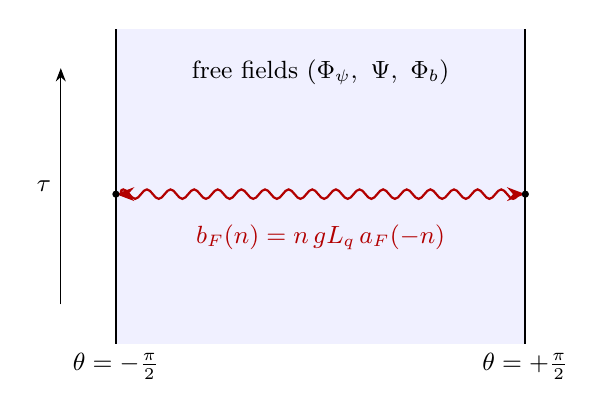
\begin{tikzpicture}[scale=1.0,>=Stealth]
\fill[blue!6] (-2.6,0) rectangle (2.6,4);
\draw[thick] (-2.6,0) -- (-2.6,4);
\draw[thick] (2.6,0) -- (2.6,4);
\node[below] at (-2.6,0) {\small $\theta=-\frac{\pi}{2}$};
\node[below] at (2.6,0) {\small $\theta=+\frac{\pi}{2}$};
\draw[->] (-3.3,0.5) -- (-3.3,3.5) node[midway,left] {\small $\tau$};
\node at (0,3.45) {\small free fields $(\Phi_\psi,\ \Psi,\ \Phi_b)$};
\draw[<->,thick,red!70!black,decorate,decoration={snake,amplitude=.6mm,segment length=3mm}] (-2.6,1.9) -- (2.6,1.9);
\node[red!70!black] at (0,1.35) {\small $b_F(n)=n\,gL_q\,a_F(-n)$};
\fill (-2.6,1.9) circle (1.3pt);
\fill (2.6,1.9) circle (1.3pt);
\end{tikzpicture}
\caption{The auxiliary system. The bulk fields on the AdS$_2$ strip are free, the cylinder time $\tau$ is the logarithm of the pair separation, and the two boundaries are the two signs of the separation. All ladder rungs sit in a constant boundary vertex connecting antipodal endpoints at equal $\tau$.}
\label{fig:strip}
\end{figure}

\section{The neutral channels and the boundary superfields}
\label{sec:neutral}

\subsection{Two scalars and a matrix condition}

An ordinary centre integral of the neutral ladder~\eqref{eq:Kmatrix} leaves a $2\times2$ problem. Its boundary-condition form was proposed in earlier unpublished work. We state it first, and derive its structure below. Take two scalars on the strip, solving $-\Phi''+m^2\sec^2\theta\,\Phi=\omega^2\Phi$, with
\begin{equation}\label{eq:scalars}
\begin{aligned}
m_\psi^2&=\mu(\mu+1),&\Phi_\psi&\to A_\psi\zeta^{-\mu}+B_\psi\zeta^{1+\mu},\\
m_b^2&=\mu(\mu-1),&\Phi_b&\to A_b\zeta^{\mu}+B_b\zeta^{1-\mu},
\end{aligned}
\end{equation}
and with parities $p$ and $1-p$. These are $\rho^2-\tfrac14$ with $\rho=\nu$ and $\rho=\delta$. With $X=(A_\psi,B_b)^T$ and $j_0=(-2\nu B_\psi,2\delta A_b)^T$, regularity gives $X=\sD_pj_0$, where
\begin{equation}\label{eq:Dp}
\sD_p(\omega)=\operatorname{diag}\left(-\frac{1}{2\nu\,\cR_{\nu,p}(\omega)},\ \frac{\cR_{\delta,1-p}(\omega)}{2\delta}\right),\qquad\sM_p=\sigma_pL_q\begin{pmatrix}2\mu&2\delta\\2\delta&0\end{pmatrix}.
\end{equation}
Then, with $\hat{\sk}_p$ the neutral kernel in the basis rescaled by $\operatorname{diag}(1,1/2\delta)$,
\begin{equation}\label{eq:khat}
\hat{\sk}_p(h)=\sD_p(h-\half)\sM_p,\qquad\sG_{g,p}=\big(\sD_p^{-1}-g\sM_p\big)^{-1},
\end{equation}
which we verified entry by entry against~\cite[(2.27)--(2.29), (2.33)--(2.35)]{Peng:2017spg}. The source-free boundary condition is $j_0=g\sM_pX$:
\begin{equation}\label{eq:bc-matrix}
-2\nu B_\psi=c\,(2\mu A_\psi+2\delta B_b),\qquad A_b=c\,A_\psi,\qquad c\equiv g\sigma_pL_q.
\end{equation}
This condition is self-adjoint for real $g$, as the boundary form $2\nu(A_{\psi1}B_{\psi2}-B_{\psi1}A_{\psi2})+2\delta(A_{b1}B_{b2}-B_{b1}A_{b2})$ vanishes on it, even though the eigenvectors of $\hat{\sk}_p$ depend on frequency. Using $\cR_{\nu,p}\cR_{\delta,1-p}=(\mu^2-\omega^2)/(4\delta\nu)$, these eigenvectors and eigenvalues are
\begin{equation}\label{eq:upm}
u_\pm(\omega)=\begin{pmatrix}1\\(\pm\omega-\mu)/2\delta\end{pmatrix},\qquad u_-:\ k_p(\omega+\half),\qquad u_+:\ k_{1-p}(\omega-\half),
\end{equation}
with $k_1=k_A$, $k_0=k_S$, in agreement with~\eqref{eq:spectra}. Undoing the rescaling, $u_\pm$ are the eigenvectors~\eqref{eq:eigvec-bottom} and~\eqref{eq:eigvec-top}.

\subsection{The scalars are components of the Dirac problem}

The first-order system~\eqref{eq:first-order} squares to the two scalar equations with $(\Phi_\psi,\Phi_b)=(v,u)$. The rotation with the opposite half-angle, $\psi=e^{(\pi/4+\theta/2)J_2}(u',v')^T$, gives a second such system with $\omega'=\Omega+\half$, now with $(\Phi_\psi,\Phi_b)=(u',v')$ and parities $(1-p,p)$. Expanding near the right endpoint gives the boundary maps
\begin{equation}\label{eq:maps}
\begin{array}{lllll}
\omega=\Omega-\half:&A_\psi=a_F,&A_b=b_F,&B_b=-\dfrac{\omega+\mu}{2\delta}a_F,&B_\psi=\dfrac{\omega-\mu}{2\nu}b_F,\\[2.5ex]
\omega'=\Omega+\half:&A_\psi=a_F,&A_b=-b_F,&B_b=\dfrac{\omega'-\mu}{2\delta}a_F,&B_\psi=\dfrac{\omega'+\mu}{2\nu}b_F.
\end{array}
\end{equation}

\begin{proposition}\label{prop:maps}
Let $\psi$ solve~\eqref{eq:HD} at frequency $\Omega$ and parity $p$, with $b_F=c\,a_F$. Then its image at $\Omega-\half$ satisfies~\eqref{eq:bc-matrix} with $c$ at parity $p$, and its image at $\Omega+\half$ satisfies~\eqref{eq:bc-matrix} with $-c$ at parity $1-p$. Their lines in the $(A_\psi,B_b)$ plane are $u_-(\Omega-\half)$ and $u_+(\Omega+\half)$.
\end{proposition}

\begin{proof}
For the first, $A_b=b_F=cA_\psi$, and $-2\nu B_\psi=-(\omega-\mu)ca_F=c(2\mu-\omega-\mu)a_F=c(2\mu A_\psi+2\delta B_b)$. For the second, with $c'=-c$: $A_b=-ca_F=c'A_\psi$, and $-2\nu B_\psi=-(\omega'+\mu)ca_F=c'(2\mu+\omega'-\mu)a_F=c'(2\mu A_\psi+2\delta B_b)$.
\end{proof}

So each root of $\cR_{F,p}(\Omega)=g\sigma_pL_q$ with $\Omega=H$ gives bosonic modes at $\omega=H-\half$ and $\omega=H+\half$, of opposite parities. With the partner Dirac mode at $-H$ and parity $1-p$, we get the one-particle energies
\begin{equation}\label{eq:energies}
(H-\half,\ H,\ H,\ H+\half),
\end{equation}
which is~\eqref{eq:multiplet} under $\omega=h-\half$. This holds for \emph{every} $g$.

The same statement holds off shell. At every complex $\omega$ and real $g$,
\begin{equation}\label{eq:ward}
\sG_{g,p}(\omega)\sM_p=\sP_-(\omega)\,\sigma_pL_q\,G^F_{g,p}(\omega+\half)+\sP_+(\omega)\,\sigma_{1-p}L_q\,G^F_{g,1-p}(\omega-\half),
\end{equation}
with $\sP_\pm$ the projectors onto $u_\pm$. So the $2\times2$ neutral correlator contains no information beyond the Dirac correlator. The neutral problem doesn't define an independent bulk theory; it is the Dirac response dressed with kinematic projectors. We verified~\eqref{eq:ward} for $q=3,5,7$ at real, complex and imaginary $\omega$.

\subsection{Boundary superfields}
\label{subsec:superfields}

The data at an endpoint assemble into two multiplets. On the strip the boundary dimensions are $\delta-\half=-\mu$ for $A_\psi$, $\delta$ for $a_F$ and $1-\mu$ for $B_b$, and likewise $\mu$, $\nu$ and $1+\mu$ for $A_b$, $b_F$ and $B_\psi$. These are long $su(1,1|1)$ multiplets $(H,H+\half,H+\half,H+1)$ with $H=\mp\mu$, which are shadows of each other in the sense $H\to-H$. Define the top components with a Weyl shift,
\begin{equation}\label{eq:tops}
\cB_-=2\delta B_b+\mu A_\psi,\qquad\cB_+=-2\nu B_\psi-\mu A_b,
\end{equation}
and the superfields
\begin{equation}\label{eq:superfields}
\Phi_-=A_\psi+\theta\,\tilde a_F+\bar\theta\,\tilde{\bar a}_F+\theta\bar\theta\,\cB_-,\qquad\Phi_+=A_b+\theta\,\tilde b_F+\bar\theta\,\tilde{\bar b}_F+\theta\bar\theta\,\cB_+,
\end{equation}
where a tilde removes the factor $e^{\mp\tau/2}$ from a fermion of definite charge, with a sign for the conjugate (\cref{subsec:surviving}). These are the $d=2$ analogue, on the cylinder, of Amsel and Marolf's boundary superfields~\cite[(3.24)]{Amsel:2008iz}, which they construct for $d=3,4,5$: their factors $(1\mp2m)$ become our $2\delta$ and $2\nu$.

The shift in~\eqref{eq:tops} is of the size expected from the superconformal map to the cylinder acting on the top component of a field of dimension $\mp\mu$, namely $-H$ times the bottom component, although we fix it here by the computation below rather than by carrying out that map. With it, a short computation shows that~\eqref{eq:bc-matrix} and~\eqref{eq:bc-dirac} are together the single statement
\begin{equation}\label{eq:bc-super}
\boxed{\ \Phi_+=c\,\Phi_-\ }
\end{equation}
This has the form of the linear condition of~\cite{Amsel:2008iz}, with constant $q=1/c$. The entry $2\mu$ of $\sM_p$, which might have looked like an accident of the reduction, is just the Weyl shift.

The boundary action is correspondingly simple. Let $S_E$ be the Euclidean free action, with the boundary terms that make its on-shell variation linear in $\delta A_\psi$, $\delta B_b$, $\delta a_F$ and $\delta\bar a_F$. Then, at the right endpoint,
\begin{equation}\label{eq:flux}
\delta S_E=\int d\tau\,d^2\theta\,\Phi_+\delta\Phi_-=\int d\tau\,\big[j_0\cdot\delta X+b_F\delta\bar a_F-\bar b_F\delta a_F\big],\qquad\int d^2\theta\,\theta\bar\theta=1.
\end{equation}
For the scalars, the Weyl shifts cancel in $A_b\delta\cB_-+\cB_+\delta A_\psi=j_0\cdot\delta X$, and the coefficients $2\nu$, $2\delta$ are those of the conserved Wronskians of the two scalars. For the fermion, $\sqrt{-g}\,\bar\Psi\gamma^\theta\delta\Psi=\bar u\delta v-\bar v\delta u$, which tends to $\bar b_F\delta a_F-\bar a_F\delta b_F$. Adding the boundary term $\int dt\,\bar a_Fb_F$, which removes $\delta b_F$, and continuing with $S_E=-\int d\tau\,\mathcal L$, gives the fermion terms in~\eqref{eq:flux}. They agree with superspace only because of the sign in $\tilde{\bar a}_F$, which was fixed separately by the closure of the supercharges.

Now $X^T\sM_pX=2\sigma_pL_q\,A_\psi(\mu A_\psi+2\delta B_b)=2\sigma_pL_q\,A_\psi\cB_-$, so the quadratic term generating~\eqref{eq:bc-matrix} is one component of a superpotential,
\begin{equation}\label{eq:superpotential}
S_{\rm bdy}=-\frac c2\int d\tau\,d^2\theta\,\Phi_-^2=\int d\tau\,\Big[-\frac g2X^T\sM_pX+c\,\bar a_Fa_F\Big].
\end{equation}
\emph{The double-trace term is a superpotential}, and its fermion component is a boundary mass. Stationarity is immediate,
\begin{equation}
\delta(S_E+S_{\rm bdy})=\int d\tau\,d^2\theta\,\big(\Phi_+-c\,\Phi_-\big)\delta\Phi_-,
\end{equation}
which gives~\eqref{eq:bc-super} in all components. This is a real check of the structure: \eqref{eq:bc-matrix} and~\eqref{eq:bc-dirac} were found separately from the ladders, and one superpotential now produces both, with the same $c$ and the same sign. At $c=0$ and $c=\infty$ we recover the two supersymmetric single-trace conditions, $\Phi_+=0$ and $\Phi_-=0$, the analogues of Thong's Neumann and Dirichlet conditions.

\section{How much bulk supersymmetry survives}
\label{sec:susy}

Thong's Robin condition breaks $2d$ AdS isometries while leaving the four-point data intact. We now ask the same question of the supercharges.

\subsection{The free multiplet}

Take the action on the strip,
\begin{equation}\label{eq:action}
S=\int d^2x\sqrt{-g}\left[\half\Phi_b\big(\Box-\mu(\mu-1)\big)\Phi_b+\half\Phi_\psi\big(\Box-\mu(\mu+1)\big)\Phi_\psi+\bar\Psi(\gamma^a\nabla_a-\mu)\Psi\right],
\end{equation}
with $\bar\Psi=\Psi^\dagger\sigma_1$ and $\gamma_3=\gamma^0\gamma^1$. The Killing equation $\nabla_a\epsilon=\half\gamma_a\epsilon$ has the solutions (compare~\cite[(A.7)]{Correa:2019rdk}, in other conventions)
\begin{equation}\label{eq:killing}
\epsilon_A=\zeta^{-1/2}\begin{pmatrix}\cos(\frac\pi4+\frac\theta2)\\ \cos(\frac\pi4-\frac\theta2)\end{pmatrix}e^{-it/2},\qquad\epsilon_B=\zeta^{-1/2}\begin{pmatrix}-\cos(\frac\pi4+\frac\theta2)\\ \cos(\frac\pi4-\frac\theta2)\end{pmatrix}e^{+it/2},
\end{equation}
giving four real supercharges with parameters $\epsilon$ and $\bar\epsilon$. For any Killing $\epsilon$ and any function $\Phi$,
\begin{equation}\label{eq:intertwine}
\begin{aligned}
(\gamma^a\nabla_a-\mu)\big(\gamma^a\partial_a+\mu\big)\Phi\,\epsilon&=\big(\Box-\mu(\mu-1)\big)\Phi\,\epsilon,\\
(\gamma^a\nabla_a-\mu)\,\gamma_3\big(\gamma^a\partial_a-\mu\big)\Phi\,\epsilon&=-\gamma_3\big(\Box-\mu(\mu+1)\big)\Phi\,\epsilon.
\end{aligned}
\end{equation}
Consequently~\eqref{eq:action} is invariant under
\begin{equation}\label{eq:susy}
\begin{aligned}
\delta\Psi&=-\big[(\gamma^a\partial_a+\mu)\Phi_b+\beta\,\gamma_3(\gamma^a\partial_a-\mu)\Phi_\psi\big]\epsilon\ \equiv\ -M(\beta)\,\epsilon,\\
\delta\Phi_b&=\bar\Psi\epsilon+\bar\epsilon\Psi,\qquad\delta\Phi_\psi=-\beta\,\bar\Psi\gamma_3\epsilon+\bar\beta\,\bar\epsilon\gamma_3\Psi,
\end{aligned}
\end{equation}
for \emph{any} constant $\beta$. These are symmetries of the free theory. Closure selects $\beta$. Acting on $\Phi_b$,
\begin{equation}
[\delta_1,\delta_2]\Phi_b=\bar\epsilon_1\big(M-\bar M\big)\epsilon_2-(1\leftrightarrow2),\qquad M-\bar M=2\gamma^a\partial_a\Phi_b+(\beta+\bar\beta)\gamma_3(\gamma^a\partial_a-\mu)\Phi_\psi,
\end{equation}
where $\bar M=\sigma_1M^\dagger\sigma_1$. The cross term vanishes if and only if $\beta$ is imaginary, and the same normalization on $\Phi_\psi$ requires $|\beta|=1$. So there are \emph{two} embeddings of the superalgebra,
\begin{equation}
\beta=\pm i,
\end{equation}
exchanged by $\Phi_\psi\to-\Phi_\psi$. In each, the anticommutators give AdS$_2$ Killing vectors,
\begin{equation}\label{eq:vectors}
(\epsilon_A,\bar\epsilon_A),\ (\epsilon_B,\bar\epsilon_B)\to\partial_t,\qquad(\epsilon_A,\bar\epsilon_B)\to E_+,\qquad(\epsilon_B,\bar\epsilon_A)\to E_-,
\end{equation}
with $E_\pm=e^{\mp it}(i\sin\theta\,\partial_t\mp\cos\theta\,\partial_\theta)$, which take $\omega\to\omega\pm1$ on $e^{-i\omega t}$. On the fermion, closure gives on-shell
\begin{equation}\label{eq:closure-psi}
\{q(\epsilon_Y),\bar q(\bar\epsilon_X)\}\Psi=-2\mathcal L_\xi\Psi+\alpha\,\Psi,\qquad\alpha=+1\ (AA),\quad-1\ (BB),\quad0\ (AB,BA),
\end{equation}
with $\mathcal L_\xi$ the spinor Lie derivative, and $\{q,q\}=0$. The term in $\alpha$ is the R-rotation. So the free theory has $su(1,1|1)$ symmetry, of dimension $4|4$, with bosonic generators $\partial_t,E_\pm,J_0$, where $J_0$ rotates $\Psi$. The field content $(\Phi_\psi,\Psi,\Phi_b)$ is a long multiplet with real, neutral scalars of different masses, not the chiral multiplet with a complex scalar considered in~\cite{Correa:2019rdk}.

\subsection{The bilinears}

The maps of \cref{prop:maps} are these variations. With $\epsilon_A$, $\bar\epsilon_A\Psi$ has frequency $\Omega-\half$, and with $\epsilon_B$, $\bar\epsilon_B\Psi$ has frequency $\Omega+\half$. On modes, one finds
\begin{equation}\label{eq:bilinears}
(\Phi_b,\Phi_\psi)=(u,v)=(\bar\epsilon_A\psi,\ -i\,\bar\epsilon_A\gamma_3\psi),\qquad(\Phi_b,\Phi_\psi)=(v',u')=(-\bar\epsilon_B\psi,\ -i\,\bar\epsilon_B\gamma_3\psi),
\end{equation}
stripped of the factors of $\zeta$ and the phases of time. The relative sign differs between $A$ and $B$. In~\eqref{eq:susy}, the $\bar\epsilon$ terms have the ratio $\Phi_\psi:\Phi_b$ fixed by $\bar\beta$. Therefore:

\begin{itemize}
\item the first of~\eqref{eq:bilinears} is the variation under $\bar\epsilon_A$ with $\beta=+i$;
\item the second is the variation under $\bar\epsilon_B$ with $\beta=-i$.
\end{itemize}
In a \emph{single} embedding, say $\beta=+i$, the $\bar\epsilon_B$ image is $(\Phi_b,\Phi_\psi)=(-v',u')$. Its line is $B_b/A_\psi=-(\omega'-\mu)/2\delta$, the opposite of the $u_+$ line allowed by~\eqref{eq:bc-matrix}. This is the crux of the breaking.

\subsection{The surviving charges}
\label{subsec:surviving}

Define, in the embedding $\beta=+i$, $q_A$ with parameter $\epsilon_A$ and $\bar q_A$ with parameter $\bar\epsilon_A$. In~\eqref{eq:susy} the parameter $\epsilon$ stands to the right of the odd fields and $\bar\epsilon$ to the left. We move both to the left and strip them off, so that $q_A$ and $\bar q_A$ act as graded derivations. Let the twisted fermions be $\tilde a_F=e^{\tau/2}a_F$ and $\tilde{\bar a}_F=-e^{-\tau/2}\bar a_F$ on the Euclidean cylinder, and the same for $b_F$, where the minus sign absorbs the one from moving $\epsilon$ past $\bar\Psi$. Evaluating~\eqref{eq:susy} at the boundary on modes of free frequency, which carry generic boundary data, we find that the charges act on the data of \cref{subsec:superfields} as
\begin{equation}\label{eq:boundary-susy}
\begin{aligned}
q_A:&\quad\delta A=\tilde{\bar a},\quad\delta\tilde a=\partial_\tau A+\cB,\quad\delta\cB=-\partial_\tau\tilde{\bar a},\quad\delta\tilde{\bar a}=0,\\
\bar q_A:&\quad\delta A=\tilde a,\quad\delta\tilde{\bar a}=\partial_\tau A-\cB,\quad\delta\cB=\partial_\tau\tilde a,\quad\delta\tilde a=0,
\end{aligned}
\end{equation}
with the same form on $(A_\psi,\tilde a_F,\cB_-)$ and on $(A_b,\tilde b_F,\cB_+)$. The normalization is exactly 1 in~\eqref{eq:susy}. The sign in $\tilde{\bar a}_F$ is needed: with the opposite one, $\{q_A,\bar q_A\}A$ would be $2\cB$. These are the supercharges of ordinary flat-time $\cN=2$ quantum mechanics, with $q_A^2=\bar q_A^2=0$ and
\begin{equation}\label{eq:twisted}
\{q_A,\bar q_A\}=2\partial_\tau\ \text{ on twisted fields, which is }-2H_{\rm tw}\ \text{ on }e^{-H_{\rm tw}\tau},\quad H_{\rm tw}=L_0-\half J_0,
\end{equation}
with $J_0=+1$ on $\Psi$, as in~\eqref{eq:closure-psi} at $\alpha=+1$. A boson of frequency $\omega$ and a fermion of frequency $\Omega=\omega+\half$ have the same twisted energy. In terms of the boundary superconformal generators, $q_A$ and $\bar q_A$ have the weights of $G_{-1/2}$ and $\bar G_{+1/2}$, whose anticommutator is $2L_0$ up to a multiple of $J_0$.

\begin{proposition}\label{prop:breaking}
For real $g\neq0$, the boundary condition~\eqref{eq:bc-super} is invariant under $\partial_\tau$, $J_0$, and $q_A,\bar q_A$. It is not invariant under $E_\pm$ or $q_B,\bar q_B$. So, in the embedding $\beta=+i$, the largest subalgebra of $su(1,1|1)$ that survives is
\begin{equation}\label{eq:breaking}
su(1,1|1)\ \longrightarrow\ u(1|1)=\big\{\,q_A,\ \bar q_A;\ L_0,\ J_0\,\big\},\qquad 4|4\to2|2.
\end{equation}
In the embedding $\beta=-i$, the same holds with $A\leftrightarrow B$.
\end{proposition}

\begin{proof}
By~\eqref{eq:boundary-susy}, $q_A,\bar q_A$ act identically on $\Phi_-$ and $\Phi_+$, so they preserve $\Phi_+=c\,\Phi_-$ for constant $c$. The breaking of $E_+$ follows from the transformation of~\eqref{eq:bc-matrix}. It maps parity $p$ to $1-p$, and $\sM_{1-p}=-\sM_p$, so its second component has the mismatch $-2g\omega(\sM_p)_{21}(X_0)_1e^{-(\omega+1)\tau}$, as found in the earlier work. The breaking of $q_B$ follows from the line argument above, since an image with the wrong sign doesn't satisfy~\eqref{eq:bc-matrix} unless $A_\psi=0$ or $\omega'=\mu$. It also follows from the algebra, since if $q_B,\bar q_B$ together with $q_A,\bar q_A$ were preserved then so would be $E_\pm$, by~\eqref{eq:vectors}.
\end{proof}

We confirmed this on explicit normal modes, and the mismatch for $E_+$ on bulk mode functions. The images under $(\bar\epsilon_A,\beta=+i)$ and $(\bar\epsilon_B,\beta=-i)$ satisfy~\eqref{eq:bc-matrix} with residuals of order $10^{-19}$ in 20-digit arithmetic, for $q=3,5$ and $g=0.7,1$. The image under $(\bar\epsilon_B,\beta=+i)$ violates it by order 10. On a generic pair of scalars, the boson-to-fermion maps in~\eqref{eq:boundary-susy} hold with normalization 1, to working precision, and so do the fermion-to-boson maps on Dirac modes of free frequency.

\Cref{tab:breaking} summarizes the pattern, and \cref{fig:multiplet} shows the action on a multiplet.

\begin{table}[t]
\centering
\renewcommand{\arraystretch}{1.2}
\begin{tabular}{@{}llcc@{}}
\toprule
Generator & Action on the cylinder & $g=0$ & $g\neq0$\\
\midrule
$L_0$ & $\partial_\tau$ & preserved & preserved\\
$J_0$ & phase of $\Psi$ & preserved & preserved\\
$E_\pm$ & $\omega\to\omega\pm1$, flips parity & preserved & \textbf{broken}\\
$q_A,\bar q_A$ & $\omega\to\omega\pm\half$, keeps parity & preserved & preserved\\
$q_B,\bar q_B$ & $\omega\to\omega\pm\half$, flips parity & preserved & \textbf{broken}\\
\bottomrule
\end{tabular}
\caption{The fate of $su(1,1|1)$ in the embedding $\beta=+i$. Compared with Thong's $sl(2,\mathbb R)\to\mathbb R$, half of the supercharges survive in addition. The R-charge is preserved since~\eqref{eq:bc-super} is homogeneous.}
\label{tab:breaking}
\end{table}

\begin{figure}[t]
\centering
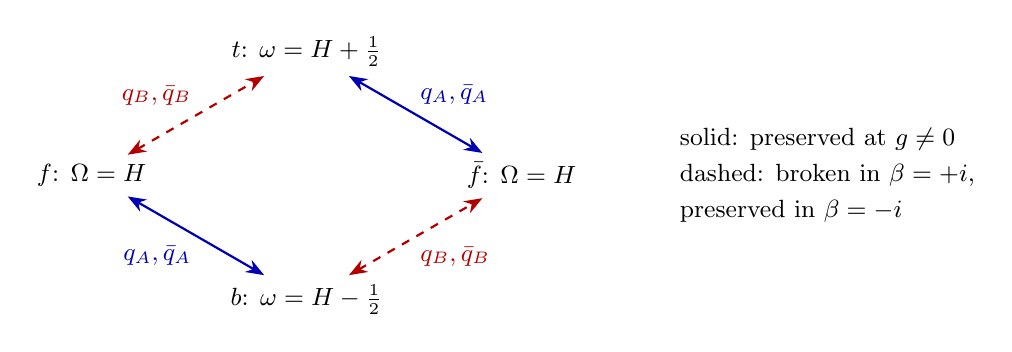
\begin{tikzpicture}[>=Stealth,scale=1.05]
\node (b) at (0,0) {\small $b$: $\omega=H-\half$};
\node (f) at (-2.6,1.5) {\small $f$: $\Omega=H$};
\node (fb) at (2.6,1.5) {\small $\bar f$: $\Omega=H$};
\node (t) at (0,3) {\small $t$: $\omega=H+\half$};
\draw[<->,thick,blue!70!black] (b) -- node[midway,below left,xshift=2pt] {\small $q_A,\bar q_A$} (f);
\draw[<->,thick,blue!70!black] (fb) -- node[midway,above right,xshift=-2pt] {\small $q_A,\bar q_A$} (t);
\draw[<->,thick,red!70!black,dashed] (b) -- node[midway,below right,xshift=-2pt] {\small $q_B,\bar q_B$} (fb);
\draw[<->,thick,red!70!black,dashed] (f) -- node[midway,above left,xshift=2pt] {\small $q_B,\bar q_B$} (t);
\node[align=left] at (6.3,1.5) {\small solid: preserved at $g\neq0$\\[1pt]\small dashed: broken in $\beta=+i$,\\[1pt]\small preserved in $\beta=-i$};
\end{tikzpicture}
\caption{One multiplet in the auxiliary system at any $g$. The four one-particle states have energies set by a root $H$ of $gk_\alpha(H)=1$. Each solid edge is a two-dimensional representation of $u(1|1)$, with central charge $2H\mp1$.}
\label{fig:multiplet}
\end{figure}

\subsection{The other charges, and the algebra they generate}

The dashed maps of \cref{fig:multiplet} are symmetries of the boundary condition too, but in the other embedding: $q_B$ and $\bar q_B$ with $\beta=-i$ preserve~\eqref{eq:bc-matrix} for all $g$. So the system with $g\neq0$ has four odd symmetries in total, $q_A^{(+)},\bar q_A^{(+)},q_B^{(-)},\bar q_B^{(-)}$, one for each Killing parameter. They explain why the spectrum~\eqref{eq:energies} has the full shape of an $su(1,1|1)$ multiplet at every $g$, although the algebra is broken. This qualifies the phrase ``half of the supersymmetry'': no supercharge is lost in the sense of having no symmetry attached to its Killing spinor. What's lost is the closure of those symmetries on AdS$_2$ isometries. The half refers to what remains of any one $su(1,1|1)$.

They aren't a broken $su(1,1|1)$ restored, however. Whereas $\{q_A^{(+)},\bar q_B^{(+)}\}=E_+$, the mixed anticommutator $\{q_A^{(+)},\bar q_B^{(-)}\}$ annihilates the top line, and maps the bottom line to the top line with a coefficient $-4\omega$, in the normalization where these lines are the images of one Dirac mode under~\eqref{eq:bilinears}. Since this coefficient depends on the mode, the four charges do not close on a Lie superalgebra with constant structure constants and the generators listed. We have not classified what they do generate.

\subsection{Origin of the breaking, and relation to the CFT}

The Euclidean strip is the half-plane, $(x,z)=e^\tau(\sin\theta,\cos\theta)$, whose boundary is the line of relative separations $x$. So $\partial_\tau$ is dilatation of $x$, and $E_\pm$ are translation and special conformal transformation of $x$. This gives a simple explanation of Thong's pattern, in any $d$: the rung $\mathcal V(y)\propto|y|^{-2\nu}$ is a double-trace coupling with a profile that singles out $y=0$ and $y=\infty$. It preserves dilatation and rotations about the origin, and breaks the $2d$ generators that move the origin. In the present case, $\mathcal V(y)\propto\sgn(y)|y|^{-2\mu}$, with a reflection, does the same.

These bulk generators aren't the CFT's pair generators, a point stressed in~\cite{Thong:2026}: bulk $E_\pm$ moves between families, while the CFT's $P_{12},K_{12}$ move within one. The same applies to supercharges. One relation does hold. By~\eqref{eq:boundary-susy}, $\delta\tilde a_F=\partial_\tau A_\psi+\cB_-$, and in terms of the original bilocal this combination is $f_b+\partial_xf_\psi$. So the condition $\delta\tilde a_F=0$ is the zero-supermomentum relation~\eqref{eq:component-relation}, and $q_A$ on the neutral fields has the same kernel as the CFT's total supertranslations. That is a matching of kernels, not an identification of charges: both $G_{-1/2}$ and $\bar G_{-1/2}$ have this kernel, and they anticommute on functions of $x$, unlike any pair of the bulk charges above that we have compared. We have not worked out the map. It is complicated by the reflection in the rung, as the reduced component covariance carries a factor $\sigma_p$ relative to $\sG_{g,p}$ (\cref{eq:cov-norm}).

None of this means that the CFT data lose their supersymmetry. The four-point function of \cref{sec:fourpoint} is organized by $su(1,1|1)$ superblocks at all $g$. It is the auxiliary bulk description that has less symmetry than the data it encodes, just as Thong's scalar has less than $SL(2,\mathbb R)$ acting on the bulk while reproducing conformal data.

\subsection{Comparison with earlier boundary-condition analyses}
\label{subsec:compare}

Amsel and Marolf~\cite{Amsel:2008iz} classify supersymmetric multi-trace conditions for scalar multiplets in AdS$_d$, $d=3,4,5$. Our results share their main features: supersymmetric conditions relate two distinct scalars, and linear conditions generically keep half of the supercharges. They note that the scalar--fermion mass relation holds in $d=2$ as well. There are two differences. Their preserved subalgebra is boundary Poincaré, closing on $P$, and their coupling is dimensionful, so it breaks dilatations. Ours closes on the twisted Hamiltonian $L_0-\half J_0$, with translations broken and dilatations preserved. In short, their condition is $\Phi_-=q\Phi_+$ in flat space with a constant, and ours is the same on the cylinder, which in flat space is a position-dependent and reflecting coupling.

Correa et al.~\cite{Correa:2019rdk} treat massless multiplets in AdS$_2$. Their Type I condition $\chi\alpha-\beta=0$ also keeps 2 of 4 supercharges and breaks scale invariance. Their Type II, with a derivative in the scalar condition and an algebraic fermion condition, keeps all 4 for $m=0$. We have not examined whether a massive analogue of Type II exists for $\Phi_\pm$, which would change the conclusions of \cref{prop:breaking} for a modified boundary theory, though not for the ladder data.

\section{Unitarity, the threshold $g_*$, and the meaning of $g$}
\label{sec:stability}

\subsection{A BPS bound}

For real $g$, the scalar problem is self-adjoint (\cref{sec:neutral}), and it has no tachyons: $\omega=iy$ with real $y\neq0$ would need $\sigma_pL_qD_\psi(\mu\pm iy)$, with $D_\psi$ real and nonzero, to equal the real number $1/g$, which is impossible. So $\omega^2\ge0$ for all real $g$, unlike Thong's AR model, where $\omega^2$ goes negative beyond a critical coupling~\cite{Thong:2026}.

The surviving algebra says more. The rotation in~\eqref{eq:first-order} is orthogonal, so $\psi^T\psi=u^2+v^2$ pointwise, and the Klein--Gordon norm of the image of a Dirac mode is
\begin{equation}\label{eq:norm}
2\omega\int d\theta\,(u^2+v^2)=2\omega\,\|\psi\|^2=(2\Omega-1)\,\|\psi\|^2.
\end{equation}
This is the central charge of~\eqref{eq:twisted}. If $\omega=H-\half>0$, the bosonic image has positive norm, so its coefficient in the field is an annihilation operator. Every charge then has the form $a^\dagger a$, and annihilates the Fock vacuum. The bound $\omega\ge0$ is saturated at $H=\half$. It is a condition for the invariance of that vacuum, not for unitarity of the auxiliary system, whose stationary quantization has a positive norm at every $g$ (see below).

Numerically, the only root that reaches $H=\half$ for $0<g\le1$ is the lowest $S$-branch root, which grows from $H=\delta$ at $g=0$ to $H=1$ at $g=1$, as shown in \cref{fig:spectrum}. It does so at
\begin{equation}\label{eq:gstar}
g_*=\frac{1}{k_S(\half)},\qquad g_*=0.21784,\ 0.34729,\ 0.39485\quad\text{for }q=3,5,7.
\end{equation}
This is where the lowest $p=0$ boson has zero frequency.

\subsection{Vacuum energy}

Summing the zero-point energies multiplet by multiplet, with bosons $\tfrac12|\omega|$ and each Dirac mode $-\tfrac12|\Omega|$, gives
\begin{equation}\label{eq:vacuum}
E_{\rm vac}(H)=\frac{|H-\half|+(H+\half)}{2}-H=
\begin{cases}0,&H\ge\half,\\ \half-H,&H<\half.\end{cases}
\end{equation}
So at $g>g_*$, including the physical point, each multiplet contributes zero, and the Fock vacuum is invariant under $q_A,\bar q_A$. We sum per multiplet, and don't address regularization of the full series.

The algebra confirms this, and shows what happens at $g<g_*$. Take the doublet of \cref{fig:multiplet} containing the lowest boson, with $a$ the annihilation operator of the boson at frequency $|\omega|$ and $f$ that of the Dirac mode at energy $H$. For $\omega>0$, the charge that lowers $L_0$ by $\half$ is $\bar Q=\sqrt{2\omega}\,a^\dagger f$. For $\omega<0$, the image $e^{-i\omega t}=e^{+i|\omega|t}$ has negative norm, so its coefficient in the field is a creation operator, and instead $\bar Q=\sqrt{2|\omega|}\,af$. Then, with $Q=\bar Q^\dagger$,
\begin{equation}\label{eq:fock}
\half\{Q,\bar Q\}=|\omega|\,(N_a-N_f+1)=L_0-\half J_0,\qquad L_0=E_{\rm vac}+|\omega|N_a+HN_f,\quad J_0=N_f,
\end{equation}
which holds exactly when $E_{\rm vac}=|\omega|=\half-H$, as in~\eqref{eq:vacuum}. So the vacuum energy is the constant in the algebra. Two things follow at $g<g_*$:
\begin{itemize}
\item The Fock vacuum, which is the lowest state of $L_0$, isn't invariant: $Q|0\rangle\neq0$, and $\langle0|\{Q,\bar Q\}|0\rangle=2E_{\rm vac}>0$.
\item The state with $N_a=0$, $N_f=1$ \emph{is} invariant. It has $L_0=\half$ and $J_0=1$, so $L_0-\half J_0=0$. It is a BPS state, and the lowest state of the twisted Hamiltonian.
\end{itemize}
So whether to call this spontaneous breaking depends on which Hamiltonian defines the vacuum. In terms of $L_0$, the generator of cylinder time, the ground state isn't supersymmetric. In terms of $L_0-\half J_0$, the only energy in the surviving algebra, it is, in the sector of R-charge 1. The reduced ladder of \cref{sec:fourpoint} uses the Fock vacuum. We haven't identified a role for the BPS state in the CFT. The pair $(\bar f,t)$ has twisted energy $H+\half>0$ and plays no part in this. The same computation for $q_B^{(-)},\bar q_B^{(-)}$ exchanges $f$ and $\bar f$, so no Fock state is invariant under the charges of both embeddings.

\subsection{Two quantizations below $g_*$}

At $g=0$, $\Phi_\psi$ in the even sector has the mode $\omega=-\mu$. This is Thong's condition $a+J>0$ failing, since $a+J=\delta-\half=-\mu$. In representation theory this is the lowest state of the long multiplet with $H=-\mu<0$. There are two options, and they differ:
\begin{itemize}
\item The \emph{continued} covariance keeps the $su(1,1|1)$ covariance of the reduced seed, with a growing exponential of negative coefficient, $w(-\mu)e^{\mu|\tau|}$, $w(-\mu)=-w(\mu)<0$, where $w(\omega)=1/(2\nu\cR'_{\nu,0}(\omega))$. Its norm isn't positive. This agrees with non-unitarity of the multiplet: $\|G_{-1/2}\ket{H}\|^2\propto2H<0$.
\item The \emph{stationary} covariance has the positive decaying mode $w(\mu)e^{-\mu|\tau|}$, but no $su(1,1|1)$ invariance.
\end{itemize}
They have the same meromorphic response, and differ by a homogeneous solution,
\begin{equation}\label{eq:homogeneous}
G^{\rm cont}(\tau)-G^{\rm stat}(\tau)=-2w(\mu)\cosh(\mu\tau),
\end{equation}
which we checked for $q=3,5$. At $g>g_*$ the question disappears, because all modes have $\omega>0$. At the physical point, the reduced ladder computed directly from the literature's four-point function has exactly the stationary modes and weights, in the entries and range tested (\cref{subsec:reduced-cov}). So no continuation in $g$ through $g_*$ is needed to define the physical system.

\subsection{The four-point function doesn't see $g_*$}

$g_*$ isn't a phase transition of the correlator on $0<z<1$. In the superblock expansion of \cref{sec:fourpoint}, poles sit at $\pm H$ and never pinch the contour, since $H\ge\delta>0$ throughout. We confirmed that~\eqref{eq:reconstruction} and the root sum agree at $g=0.15<g_*$ for $q=3$, as at larger $g$. What fails at $g_*$ is the ordinary centre integral of a component block, which needs $\mathrm{Re}\,h>\half$, because its tail is $|u|^{-2h}$. So $g_*$ is a boundary of validity for the reduced bosonic description. The Dirac description, with $\Omega=H$ and weight $\delta$, has no such boundary, and nor does the super-centre integral of \cref{subsec:supercentre}, which converges for $H>-\half$ and gives the Dirac propagator at every $g$.

\begin{figure}[t]
\centering
\begin{tikzpicture}
\begin{axis}[width=0.72\textwidth,height=0.42\textwidth,xlabel={$g$},ylabel={$H$},xmin=0,xmax=1,ymin=0,ymax=3,
 legend style={at={(0.98,0.72)},anchor=north east,font=\small,draw=none,fill=white,fill opacity=0.8,text opacity=1},tick label style={font=\small},label style={font=\small}]
\addplot[thick,blue!70!black] table[x=g,y=HS0,col sep=space,comment chars={\#}] {../../../results/data/paper/spectrum_q3.dat};
\addlegendentry{$S$-branch, lowest}
\addplot[thick,red!70!black,dashed] table[x=g,y=HA0,col sep=space,comment chars={\#}] {../../../results/data/paper/spectrum_q3.dat};
\addlegendentry{$A$-branch, lowest}
\addplot[thick,blue!70!black,dotted] table[x=g,y=HS1,col sep=space,comment chars={\#}] {../../../results/data/paper/spectrum_q3.dat};
\addlegendentry{$S$-branch, next}
\addplot[gray,densely dashed] coordinates {(0,0.5) (1,0.5)};
\node[font=\small,gray] at (axis cs:0.84,0.36) {$H=\tfrac12$};
\addplot[gray] coordinates {(0.21784,0) (0.21784,3)};
\node[font=\small,gray,anchor=west] at (axis cs:0.225,1.85) {$g_*$};
\addplot[only marks,mark=*,mark size=1.3pt] coordinates {(1,1)};
\end{axis}
\end{tikzpicture}
\caption{Lowest roots of $gk_\alpha(H)=1$ at $q=3$, computed from~\eqref{eq:kAkS}. Both lowest branches reach $H=1$ at $g=1$. Below $g_*$, the lowest $S$-branch root violates the bound $H\ge\half$, and the Fock vacuum isn't invariant under the surviving charges. Data: \texttt{results/data/paper/spectrum\_q3.dat}.}
\label{fig:spectrum}
\end{figure}

\subsection{A supersymmetric line of theories}
\label{subsec:line}

So far $g$ has been a formal weight. In the $\cN=0$ model, it has a microscopic meaning through conformal SYK~\cite{Gross:2017aos}, in which the kinetic term is replaced by a bilocal. The construction appears to carry over. Replace the kinetic term by
\begin{equation}\label{eq:bilocal}
S_0=\int d\mu_1d\mu_2\,\bar\Psi(1)\,K(\ket{12})\,\Psi(2),
\end{equation}
with $K$ the inverse of $\bar G=\bar b\,\sgn\ket{12}/|\ket{12}|^\delta$, and keep the superpotential. In components we expect UV propagators $\bar G_\psi$ and $\bar G_b=-\partial\bar G_\psi$, though we haven't carried out this reduction. Schwinger--Dyson is then $G_i^{-1}=\bar G_i^{-1}-\Sigma_i$, with $\Sigma_i$ as in~\cite{Peng:2017spg}. With the conformal form, and $b_\psi/\bar b_\psi=b_b/\bar b_b=r$, we have in frequency space $G_i\bar G_i^{-1}=r$ and $G_i\Sigma_i=-g$, where $g=Jb_\psi^{q-1}b_b/(Jb_\psi^{q-1}b_b)_{\rm IR}$ is the same in both equations, since the IR solution makes each product $-1$. Thus
\begin{equation}
g=1-r,
\end{equation}
which is~\cite[(C.9)]{Thong:2026} with $r=2\bar b$. All three entries of~\eqref{eq:Kmatrix} scale the same way, as $Jb_\psi^q$ at fixed $b_b/b_\psi=\delta$, so $\hat{\sk}_p\to g\hat{\sk}_p$. This is exactly the formal $g$ above. At $g<1$ the $H=1$ multiplets lift, as $k_\alpha(1)=1\neq1/g$, consistent with a nonlocal theory having no local stress tensor. We have checked neither reflection positivity nor anything beyond leading order in $1/N$, so this remains a proposal.

\section{The four-point function}
\label{sec:fourpoint}

\subsection{Superconformal reconstruction}

In the chiral--antichiral ordering, with cross ratio $0<z<1$ (the $\chi$ of~\cite{Bulycheva:2018qcp}, related to the component cross ratio of~\cite{Peng:2017spg} by $\chi_{\rm PSV}=z/(z-1)$), the normalized seed is $F_0=z^\delta$, and the normalized fermion covariance in this ordering is $-F$. The superblock is~\cite{Bulycheva:2018qcp}
\begin{equation}\label{eq:block}
\varphi_H(z)=\frac{\Gamma(H)^2}{\Gamma(2H)}z^H{}_2F_1(H,H;2H+1;z)=F_H(z)-F_{H+1}(z),
\end{equation}
with $F_h$ the $sl(2)$ block, $\cC\varphi_H=H^2\varphi_H$. A fixed transform relates it to the cylinder mode, $\cT_2e^{-Ht}=\varphi_H$, where
\begin{equation}\label{eq:T2}
(\cT_2f)(z)=2\sqrt2\int_\eta^\infty\frac{\sinh(t/2)f(t)}{\sqrt{\cosh t-\cosh\eta}}\,dt,\qquad\eta=\operatorname{arcosh}(2/z-1),
\end{equation}
and $\cC\cT_2=\cT_2\partial_t^2$ on this span. The four-point function is
\begin{equation}\label{eq:reconstruction}
F_g(z)=\int_{\cC}\frac{dH}{2\pi i}\,r_g(H)\varphi_H(z)+\frac{2\cN_\delta}{\pi}\sum_{n\ge1}\frac{k_A(n)}{1-gk_A(n)}\varphi_n(z),
\end{equation}
where $\cC$ crosses the real axis in $0<c<\delta$, and
\begin{equation}\label{eq:rg}
r_g(H)=\cN_\delta\left[\cot\frac{\pi H}{2}\,\frac{k_A(H)}{1-gk_A(H)}-\tan\frac{\pi H}{2}\,\frac{k_S(H)}{1-gk_S(H)}\right],\qquad\cN_\delta=\frac{\delta}{2\nu\tan(\pi\delta/2)}.
\end{equation}
This follows from~\cite[(4.106)]{Bulycheva:2018qcp} after the corrections of \cref{app:conventions}: send $h\to-h$ in the shadow term, and use $(1\pm\sec\pi h)/\tan\pi h=\cot\frac{\pi h}{2},\,-\tan\frac{\pi h}{2}$. Closing the contour, the integer poles cancel against the explicit sum, leaving
\begin{equation}\label{eq:roots}
F_g(z)=\sum_{k_A(H)=1/g}\frac{\cN_\delta\cot(\pi H/2)}{g^2k_A'(H)}\varphi_H(z)-\sum_{k_S(H)=1/g}\frac{\cN_\delta\tan(\pi H/2)}{g^2k_S'(H)}\varphi_H(z).
\end{equation}
We verified that~\eqref{eq:reconstruction} equals~\eqref{eq:roots} numerically at finite $g$, and that the coefficients in~\eqref{eq:roots}, together with the $F_H-F_{H+1}$ structure, reproduce the residues of~\cite[(4.26)]{Peng:2017spg} with $g$ inserted, at $g=0.7$ and $g=1$, for $q=3,5$. That is an independent derivation of the same data in components.

\subsection{The reduced component covariance}
\label{subsec:reduced-cov}

Now we can test the central claim directly, by computing the left side of Thong's identity from the literature. Let $F^{(0)}_{g,p}$ be the ordinary centre integral of the neutral correlators, projected onto unit-normalized parity harmonics, $E(\tau)=\operatorname{diag}(e^{a_\psi\tau},e^{a_b\tau})$, with $a_\psi=\delta-\half$, $a_b=\delta+\half$, and $S=\operatorname{diag}(1,1/2\delta)$. The claim, due to the earlier note, is
\begin{equation}\label{eq:cov-norm}
S\,E\,F^{(0)}_{g,p}\,E\,S=\sigma_p\ell_\psi\,\sG_{g,p},\qquad\ell_\psi=\frac{2\cdot4^{-\nu}}{Jb_\psi^{q-2}}.
\end{equation}
We can evaluate both sides independently. For the left side, we use the four-point functions of~\cite[(4.26), (4.35)]{Peng:2017spg}, with $g$ inserted by the geometric series, and Thong's reduction of a block~\cite[(C.8)]{Thong:2026},
\begin{equation}\label{eq:P}
(\mathsf PB_h)(\tau)\equiv\int_{-\infty}^\infty du\,B_h\Big(\frac{1}{u^2-\sinh^2(\tau/2)}\Big)=\cI(h)\,e^{-(h-\frac12)|\tau|},\qquad\cI(h)=\frac{\pi\tan(\pi h/2)}{(2h-1)\cN(h)},
\end{equation}
with $\cN(h)=\Gamma(h)^2/2\Gamma(2h)$. In the even sector, which~\cite{Thong:2026} doesn't need, we use $\Phi^a_h$ of~\cite{Peng:2017spg} with the same piecewise prescription. We find by quadrature that
\begin{equation}\label{eq:Ia}
\cI_a(h)=\frac{\pi\cot(\pi h/2)}{(2h-1)\cN(h)},
\end{equation}
which is what Thong's weights give under $\tan\frac{\pi h}{2}\to\tan\frac{\pi(h-1)}{2}$, as $\cos\pi\omega+\tan\frac{\pi(h-1)}{2}\sin\pi\omega=\cot\frac{\pi h}2$. The tangents cancel against the measure, and for the $\psi\bar\psi\psi\bar\psi$ entry the sum over blocks becomes
\begin{equation}\label{eq:PF}
(\mathsf PF_{g,p})(\tau)=\mp2\sum_{h_*}\Res_{h=h_*}\frac{k_0^{\psi}(h)}{D_p(h)}\,e^{-(h_*-\frac12)|\tau|},\qquad D_p(h)=(1-gk_p(h))(1-gk_{1-p}(h-1)),
\end{equation}
with upper sign for $p=1$, and $k_0^\psi$ the seed overlaps $k_0^{\psi,s}$ for $p=1$ and $k_0^{\psi,a}$ for $p=0$ of~\cite[(4.10), (4.11)]{Peng:2017spg}. For the right side, we use the residues of $\sG_{g,p}$ from~\eqref{eq:khat}.

The two agree at every root with $\omega<4$, for $q=3,5$, at $g=0.5,0.9,0.99,1$ when $p=1$, and at $g=0.9,0.99,1$ when $p=0$, including the exceptional roots below. The other three entries agree as well, at every root with $\omega<4$ of each parity, for $q=3,5$ and $g=0.9,1$, again including the exceptional roots, subject to one point of normalization. The matrix~\cite[(4.25)]{Peng:2017spg} acts on coefficients of bilocals with no amplitudes extracted, so the normalized correlators of a column must carry the amplitude $b_j^2$ of the $(3,4)$ pair in both rows. If the off-diagonal correlators were normalized literally by $G_i(\tau_{12})G_j(\tau_{34})$, the two off-diagonal entries would differ by a factor $\delta^2$, which violates the symmetry $F_{21}=F_{12}$ of the reduced covariance. With the column normalization that symmetry holds exactly.

As a separate test of the reduction formula, a direct numerical centre integral of the odd part of the seed, $\frac12[\sgn\frac{\chi}{1-\chi}|\frac{\chi}{1-\chi}|^\delta-\sgn\chi|\chi|^\delta]$, agrees with~\eqref{eq:PF} at $g=0$. The even part has no such test, since its centre integral diverges. We haven't tested the reduction of the summed series.

\subsection{The super-centre integral}
\label{subsec:supercentre}

The ordinary centre integral imposes only $L_1=0$, and so it keeps both the bottom and the top component of each multiplet (\cref{sec:cylinder}). Integrating over the whole supertranslation orbit of a pair imposes all the conditions of \cref{prop:cylinder}. We now show that this turns the four-point function directly into the Dirac propagator, with one exponential per superblock.

\paragraph{The integral.} Write the chiral--antichiral four-point function as $G(\ket{12})G(\ket{34})\,\mathcal F_g(z)$, with $z=\ket{12}\ket{34}/(\ket{14}\ket{32})$, $\mathcal F_g$ given by~\eqref{eq:reconstruction} on $0<z<1$, and $G$ the superfield propagator, whose bottom component is $G_\psi$. This form is general. Chirality leaves $4|4$ coordinates, on which $su(1,1|1)$ acts with rank $3|4$, so $z$ is the only invariant and there is no nilpotent one. Move the pair $(12)$ along its supertranslation orbit, by the flow of $\eta G_{-1/2}+\bar\eta\bar G_{-1/2}$ and a translation $Y$,
\begin{equation}
\theta\to\theta+\bar\eta,\qquad\bar\theta\to\bar\theta+\eta,\qquad\tau\to\tau+Y-\eta\theta-\bar\eta\bar\theta,
\end{equation}
and keep $(34)$ fixed. Starting from vanishing odd coordinates, $\ket{12}=x$ and $\ket{34}=y$ don't change, while
\begin{equation}
\ket{14}=Y+s+\eta\bar\eta,\qquad\ket{32}=s-Y+\eta\bar\eta,\qquad s=\tfrac12(x+y).
\end{equation}
So $z=z_0-2s\,z_0^2\,\eta\bar\eta/xy$, where $z_0=xy/(s^2-Y^2)$ is the body. With the invariant measure $dY\,d^2\eta$ and $\int d^2\eta\,\eta\bar\eta=1$,
\begin{equation}\label{eq:Ps}
\mathsf P_sF\equiv\int dY\,d^2\eta\,F=-G(x)G(y)\,\frac{x+y}{xy}\int dY\,z_0^2\,\mathcal F'(z_0).
\end{equation}
Two things distinguish this from the ordinary centre integral. At large $|Y|$, where $\mathcal F\sim z^H$, it converges for $H>-\half$ rather than $H>\half$. At the collisions $\ket{14}=0$ and $\ket{32}=0$ its integrand is more singular, and we take the finite part, which is the same as continuing in the exponents.

The two integrals are simply related. Put $x=e^\tau n$, $y=e^{\tau'}n'$, $t=\tau-\tau'$, and use the component cross ratio $\chi=z/(z-1)$. Then $z^2\partial_z\mathcal F=-\chi^2\partial_\chi\mathcal F$, and $\partial_t\chi=\pm\frac12\sinh t\,\chi^2$ in the two sectors. Therefore
\begin{equation}\label{eq:Ps-P}
\frac{(|x||y|)^\delta}{b_\psi^2}\,\mathsf P_sF=\begin{cases}2n\,\partial_t\mathsf P_+\mathcal F/\sinh\frac t2,&n'=n,\\[0.5ex]-2n\,\partial_t\mathsf P_-\mathcal F/\cosh\frac t2,&n'=-n,\end{cases}
\end{equation}
where $\mathsf P_+=\mathsf P$ is the centre integral~\eqref{eq:P}, $\mathsf P_-$ is the same with $\chi=1/(\cosh^2\frac t2-u^2)$, and both act on $\mathcal F$ written as a function of $\chi$. The odd directions of the super-centre act as a first-order operator in cylinder time.

\paragraph{One superblock.} On $0<z<1$ the family of a root $H$ is $\varphi_H=F_H-F_{H+1}$. By~\eqref{eq:spectra}, its bottom component has parity $p$ and its top component parity $1-p$, with $p=1$ on the $A$ branch and $p=0$ on the $S$ branch. Outside $0<z<1$ we continue each component as its own family: the odd one as in~\cite[(C.4)]{Thong:2026}, and the even one with $\Phi^a_h$, as in~\eqref{eq:Ia}. Call the results $\Phi^A_H$ and $\Phi^S_H$. Since $F_h=2\cN(h)B_h$,~\eqref{eq:P} and~\eqref{eq:Ia} give, on the $A$ branch,
\begin{equation}
\mathsf P_\pm\Phi^A_H=\pi\tan\frac{\pi H}2\left[\frac{e^{-(H-\frac12)|t|}}{H-\half}\mp\frac{e^{-(H+\frac12)|t|}}{H+\half}\right],
\end{equation}
two exponentials, one for each component. Their $t$-derivatives are $-2\pi\tan\frac{\pi H}2\,e^{-H|t|}$ times $\sinh\frac t2$ and $\sgn t\cosh\frac t2$ respectively, so~\eqref{eq:Ps-P} leaves a single exponential. The $S$ branch works the same way, with $\cot$ in place of $\tan$.

\begin{proposition}\label{prop:supercentre}
For $H>-\half$, with $\theta$ the step function,
\begin{equation}\label{eq:Ps-family}
\begin{aligned}
\frac{(|x||y|)^\delta}{b_\psi^2}\,\mathsf P_s\big[GG\,\Phi^A_H\big]&=-4\pi\tan\frac{\pi H}2\,\big[\theta(t)\,n'+\theta(-t)\,n\big]\,e^{-H|t|},\\
\frac{(|x||y|)^\delta}{b_\psi^2}\,\mathsf P_s\big[GG\,\Phi^S_H\big]&=4\pi\cot\frac{\pi H}2\,\big[\theta(t)\,n+\theta(-t)\,n'\big]\,e^{-H|t|}.
\end{aligned}
\end{equation}
\end{proposition}

The derivation used the ordinary integrals, which need $H>\half$, but both sides are analytic in $H$ and~\eqref{eq:Ps} converges for $H>-\half$. So the super-centre integral of a superblock is a single exponential $e^{-H|t|}$, a single Dirac mode at $\Omega=H$, where the ordinary centre integral gives two, at $\omega=H\mp\half$. It is one-sided in $t$, as a first-order propagator must be. In the parity blocks $\theta(t)e^{-Ht}$ appears in one and $\theta(-t)e^{Ht}$, the partner pole at $-H$, in the other, as in~\eqref{eq:spectral}. The parity of the pair $(12)$ is exchanged, because the odd directions act on it as a derivative. In components, the collapse needs the bottom and the top of one Dirac pole to carry weights in the ratio $(H+\half):-(H-\half)$ in the $\psi\bar\psi\psi\bar\psi$ entry. That is what the Ward identity~\eqref{eq:ward} gives, since its $11$ entry reads $\sG_{g,p,11}(\omega)=-[G^F_{g,p}(\omega+\half)+G^F_{g,1-p}(\omega-\half)]/2\omega$.

\paragraph{The four-point function.} With the coefficients~\eqref{eq:roots}, the tangents and cotangents cancel. Each root then contributes the residue of $k_\alpha/(1-gk_\alpha)$, which by~\eqref{eq:ladder-dirac} is $\sigma_pL_q$ times a Dirac weight $w_n$. Summing,
\begin{equation}\label{eq:Ps-dirac}
\boxed{\ (|x||y|)^\delta\int dY\,d^2\eta\;F_g(1,2,3,4)=8\pi\cN_\delta L_q\,b_\psi^2\,\big(\mathfrak G_{F,g}\Pi\big)(\tau-\tau';n,n'),\ }
\end{equation}
with $\mathfrak G_{F,g}$ the Dirac propagator~\eqref{eq:ladder-position} and $(\Pi h)(\tau,n)=h(\tau,-n)$ the parity. In the normalization of~\cite{Peng:2017spg}, $8\pi\cN_\delta L_qb_\psi^2=2\ell_\psi$, the constant of~\eqref{eq:cov-norm}. In terms of the literature's data alone, a root contributes $-4\Res[(2h-1)k_0^{\psi,s}/D_1]$ on the $A$ branch and $4\Res[(2h-1)k_0^{\psi,a}/D_0]$ on the $S$ branch, with $D_p$ as in~\eqref{eq:PF}. These contain no trigonometric factor and are finite at the exceptional roots, so the cancellation of \cref{subsec:exceptional} is automatic here.

We checked~\eqref{eq:Ps-dirac} in three ways. First, at $g=0$ the seed is $\mathcal F_0=\sgn(z)|z|^\delta$, and~\eqref{eq:Ps} can be done in closed form, with $|z|^a$ in place of $|z|^\delta$ and continuing from $-\half<a<0$, where it converges. The result is $-2\delta\,[B(\half,-\delta)+B(\half+\delta,-\delta)]\,n$ times $\cosh^{-2\delta}\frac t2$ for $n'=n$, and $\sgn t\,|\sinh\frac t2|^{-2\delta}$ for $n'=-n$. This is~\eqref{eq:Ps-dirac} at $g=0$, for $q=3,5,7$. It includes the even part of the seed, whose ordinary centre integral diverges. Second,~\eqref{eq:Ps-family} holds by quadrature of the component families, at $H$ from $0.3$ to $2.4$. Third, at every root with $H<3.6$, for $q=3$ at $g=0.15,0.5,0.9,1$ and $q=5$ at $g=0.3,0.7,1$, the weights from~\cite{Peng:2017spg} equal $\mp4\pi\cN_\delta L_qw_n$, with $w_n=1/\cR_{F,p}'(H_n)$. That includes the exceptional roots, and the lowest $S$ roots with $H<\half$ for $g<g_*$.

So~\eqref{eq:Ps-dirac} is the $\cN=2$ analogue of~\cite[(3.11)]{Thong:2026} for the full four-point function. Together with~\eqref{eq:ladder-position}, it says that one Dirac field reproduces both the charged ladders, through an ordinary centre integral, and the neutral superconformal four-point function, through a super-centre integral. Unlike the ordinary reduction of the neutral components, it holds through $g_*$.

The reconstruction~\eqref{eq:reconstruction} is its inverse. Let $\cI_s(H)$ be the prefactor in~\eqref{eq:Ps-family}, $-4\pi\tan\frac{\pi H}2$ or $4\pi\cot\frac{\pi H}2$. By~\eqref{eq:rg}, $r_g(H)\,\cI_s(H)=-4\pi\cN_\delta\,k_\alpha/(1-gk_\alpha)$ on each branch. So the trigonometric factors of $r_g$ are exactly those that $\mathsf P_s$ removes, and $\cT_2$, which maps $e^{-Ht}$ to $\varphi_H$, inverts $\mathsf P_s$ family by family up to $\cI_s(H)$.

Two caveats remain, as in~\cite{Thong:2026}. The continuation of the superfamilies outside $0<z<1$ is inherited from the component families, not characterized in superspace. And we have not shown that the reduction commutes with the infinite sum over families.

\subsection{Exceptional families}
\label{subsec:exceptional}

At $g=1$ both branches reach $H=1$. For the $S$ multiplet the story is Thong's for $h=2$: the block coefficient diverges as $g\to1$, the centre integral vanishes, and the product is finite. For the $A$ multiplet the coefficient vanishes, since $c_A\propto\cot(\pi H/2)\to0$ in~\eqref{eq:roots}, yet $\sG_{1,p}$ has nonzero residues there. This looks like a contradiction with~\cite[(3.13)]{Thong:2026}, which says that the same coefficient multiplies each family before and after reduction. It isn't, as we now show.

The eigenfunctions $\Phi^s_h$ of~\cite{Peng:2017spg} have poles at odd $h$, and $\Phi^a_h$ at even $h$, with Legendre residues, where $x=(\chi-2)/\chi$:
\begin{equation}\label{eq:Phi-res}
\Res_{h=2n+1}\Phi^s_h=-2P_{2n}(x),\qquad\Res_{h=2n+2}\Phi^a_h=+2P_{2n+1}(x).
\end{equation}
We checked this for the first two values of each at $\chi>1$, and at $h=1$ also for $0<\chi<1$. These poles are cancelled by zeros of the measure, as noted for $\Psi_h$ in~\cite{Maldacena:2016hyu}. The two regions now differ, because of how the contour is closed. On $\chi>1$, one closes to the right with $\Phi_h$ itself. On $0<\chi<1$, one first uses $h\to1-h$ to replace $\Phi_h$ by the block $\propto\chi^h{}_2F_1(h,h;2h;\chi)$, which has no pole at these $h$~\cite{Maldacena:2016hyu,Peng:2017spg}. So at a root $h_*\to1$ of $D_p$, the zero of the measure removes the term on $0<\chi<1$, while on $\chi>1$ a finite contribution remains:
\begin{equation}\label{eq:step}
\frac{2h-1}{\pi\tan(\pi h/2)}\Phi^s_h\xrightarrow{h\to1}1\quad(\chi>1),\qquad\frac{2h-1}{\pi\tan(\pi(h-1)/2)}\Phi^a_h\xrightarrow{h\to2}-3P_1(x)\quad(\chi>1).
\end{equation}
In the piecewise representation of~\cite[(C.4)]{Thong:2026}, the family at $g\to1$ is therefore $\theta(\chi>1)$ or $P_1(x)\theta(\chi>1)$, times a constant. Numerically at $q=3$, $p=1$, $g=0.9999$, the family contributes $1.8\times10^{-6}$ at $\chi=0.5$ and $-0.26532$ at $\chi=1.6$, against the predicted $-\Res[k_0^{\psi,s}/D_1]=-0.26532$.

\begin{lemma}\label{lem:step}
With $\chi=1/(u^2-\sinh^2(\tau/2))$,
\begin{equation}\label{eq:step-lemma}
\mathsf P\big[\theta(\chi>1)P_n(x)\big]=\frac{2}{2n+1}e^{-(n+\frac12)|\tau|}.
\end{equation}
\end{lemma}

\begin{proof}
The region $\chi>1$ is $\sinh\frac{|\tau|}{2}<|u|<\cosh\frac\tau2$, on which $x=1-2(u^2-\sinh^2\frac\tau2)$ runs over $[-1,1]$. Changing variables gives $\int_{-1}^1P_n(x)\,dx\,(2\cosh\tau-2x)^{-1/2}$. With $t=e^{-|\tau|}$ we have $2\cosh\tau-2x=(1-2xt+t^2)/t$, so the Legendre generating function gives $(2\cosh\tau-2x)^{-1/2}=\sqrt t\sum_mt^mP_m(x)$, and orthogonality finishes the proof.
\end{proof}

For $n=0$ this is the statement that the interval has width $2(\cosh\frac\tau2-\sinh\frac{|\tau|}2)=2e^{-|\tau|/2}$, so the step function reduces exactly to the mode at $\omega=\half$. Together with~\eqref{eq:step} this reproduces~\eqref{eq:PF} at both $A$-modes. \Cref{tab:exceptional} summarizes.

\begin{table}[t]
\centering
\renewcommand{\arraystretch}{1.2}
\begin{tabular}{@{}cccccl@{}}
\toprule
Branch & $p$ & $h$ & Block coefficient, $g\to1$ & $\cI$ & Reduced weight\\
\midrule
$A$ & 1 & 1 & $\to0$ & pole & finite, nonzero\\
$A$ & 0 & 2 & $\to0$ & pole & finite, nonzero\\
$S$ & 1 & 2 & $\to\infty$ & 0 & finite, nonzero\\
$S$ & 0 & 1 & $\to\infty$ & 0 & finite, nonzero\\
\bottomrule
\end{tabular}
\caption{The $H=1$ modes. The $S$ rows are Thong's $h=2$ mechanism, and the $A$ rows are its mirror image.}
\label{tab:exceptional}
\end{table}

So in the decomposition into families, the $A$-modes are present, as a step function that vanishes on $0<\chi<1$. The chiral--antichiral reconstruction lives at $\chi_{\rm PSV}<0$, where the piecewise family also vanishes, so it can't see them. The two statements are compatible, and~\cite[(3.13)]{Thong:2026} holds, provided the family at $g=1$ is understood as this step function or as the limit $g\to1^-$. This fits the expectation of~\cite{Fu:2016vas} that the $A$ multiplet has no divergence and corresponds to operators of the IR theory.

We stress that this describes a term in a decomposition. It doesn't imply that the full correlator jumps at $\chi=1$, where the infinite sum over the other families is itself singular. We haven't examined what such a term means physically, beyond its effect on the centre integral.

\subsection{The $S$ multiplet}

The divergence as $g\to1$ reflects the soft modes, and~\cite{Bulycheva:2018qcp,Peng:2017spg} leave this multiplet aside. A definite conformal subtraction, proposed in the earlier note, is
\begin{equation}
F_{\rm sub}(z)=\lim_{g\to1^-}\left[F_g(z)-\frac{D_\delta}{1-g}\varphi_1(z)\right],\qquad D_\delta=\frac{2\cN_\delta}{\pi},
\end{equation}
and with $b_1=k_S'(1)$, $b_2=k_S''(1)$ the pole moves as $H(g)=1+(1-g)/b_1+\cdots$, leaving the finite contribution
\begin{equation}\label{eq:finite-part}
\frac{D_\delta}{b_1}\partial_H\varphi_H(z)\Big|_{H=1}+D_\delta\Big(1-\frac{b_2}{2b_1^2}\Big)\varphi_1(z),
\end{equation}
whose coefficients we checked. This is a conformal finite part, not the finite-coupling answer. A different subtraction changes the coefficient of $\varphi_1$. Its physical value requires the super-Schwarzian~\cite{Fu:2016vas}, which has not been computed in any work we have read. On the reduced side the ambiguity disappears, in the way of~\cite[(C.12)]{Thong:2026}: $\varphi_1=F_1-F_2$, and $\cI_a(1)=\cI(2)=0$. Accordingly the residues of $\sG_{1,p}$ at these modes are finite and unambiguous.

\section{Discussion}
\label{sec:discussion}

We have shown that the ladder structure of $\cN=2$ SYK reduces to a single Dirac response on the AdS$_2$ strip, with two scalars as its components in the bosonic reduction, and that a constant double-trace superpotential on the cylinder breaks the bulk superalgebra from $su(1,1|1)$ to $u(1|1)$. The spectrum retains the shape of the full multiplets at all $g$, as in Thong's case where the dimensions and OPE data survive the loss of $E_\pm$. We list what we consider the main open points.

\paragraph{The super-centre integral.} \Cref{subsec:supercentre} maps each superblock to one exponential, and the four-point function to the Dirac propagator, so one Dirac field is the $\cN=2$ replacement of Thong's single scalar at the level of four-point data. Two points remain open there. The continued superfamilies are defined through their components, and a characterization in superspace, for instance through the eigenfunctions~\cite[(4.40)]{Bulycheva:2018qcp} on $z>1$, would be more natural. And the finite part at the collisions is a prescription.

\paragraph{Term-by-term reduction.} We have not proved the analogue of~\cite[App.~C.2]{Thong:2026} for the $\cN=2$ families, ordinary or super, including the step-function families, or that the mixed $\psi$--$b$ continuation allows the required exchanges of integrals. Working with $G(\ket{12})$ directly may avoid the separate infrared and ultraviolet divergences of the fermion and boson rails.

\paragraph{A modified boundary theory.} \Cref{prop:breaking} concerns the given boundary domain. A massive analogue of the Type II condition of~\cite{Correa:2019rdk} might preserve more, at the cost of a derivative term in the scalar condition. It isn't clear that such a theory would reproduce the ladder data.

\paragraph{The physical $H=1$ coefficient.} Connecting~\eqref{eq:finite-part} to the super-Schwarzian~\cite{Fu:2016vas,Forste:2017apw} is a well-defined next computation, which the literature we have read leaves undone~\cite{Peng:2017spg,Bulycheva:2018qcp}.

\paragraph{Antipodal coupling.} The boundary vertex couples the two boundaries of global AdS$_2$ at equal time (\cref{fig:strip}). That has the form of the double-trace couplings that make wormholes traversable~\cite{Gao:2016bin,Maldacena:2018lmt}. We mention this only as a structural similarity. Here the bulk is rigid and the fields are auxiliary, and the two boundaries are the two signs of a relative separation, not two copies of a system.

\paragraph{Stepping stones.} Complex SYK at zero charge is a useful test. We find its symmetric-channel kernel~\cite{Bulycheva:2017uqj,Gu:2019jub} satisfies
\begin{equation}
k^S(h)\,\cR_{\nu,0}(h-\half)=4^{-\nu},\qquad\nu=1-\frac2q,
\end{equation}
to be compared with $k^A\cR_{\nu,1}=(q-1)4^{-\nu}$~\cite{Thong:2026}. So it is one scalar with a parity-dependent Robin coefficient, with a mode at $h=1$ for the $U(1)$ charge and $a+J=2/q-\half<0$ for $q>4$. It is the simplest system where the even-sector issues of \cref{sec:stability} arise without mixing. $\cN=1$ tests something else, because it has an odd relative coordinate.

\paragraph{Beyond this paper.} Nonzero charge~\cite{Gu:2019jub,Heydeman:2022lse} would need a $\theta$-dependent mixing. Higher-point data remain out of reach. Thong's caveat stands: this construction concerns four-point data, not an equivalence of theories.

\appendix
\section{Labels and printed discrepancies}
\label{app:conventions}

\paragraph{Labels.} The conventions in the literature collide, as follows.

\begin{center}
\small
\renewcommand{\arraystretch}{1.2}
\begin{tabular}{@{}llll@{}}
\toprule
This paper & \cite{Peng:2017spg}, kernels & \cite{Peng:2017spg}, four-point & \cite{Fu:2016vas}\\
\midrule
$p=1$ (odd fermion pair) & $k^{a,\pm}$ & $f^s,\Phi^s$ & \\
$p=0$ (even fermion pair) & $k^{s,\pm}$ & $f^a,\Phi^a$ & \\
$k_A(H)$ & $k^{a,+}(H)=k^{a,d}(H+\half)=k^{s,-}(H+1)$ & & $k_a(H+\half)$\\
$k_S(H)$ & $k^{s,+}(H)=k^{s,d}(H+\half)=k^{a,-}(H+1)$ & & $k_s(H+\half)$\\
\bottomrule
\end{tabular}
\end{center}

Also, the $\chi$ of~\cite{Bulycheva:2018qcp} is our $z$, while the $\chi$ of~\cite{Peng:2017spg} is $z/(z-1)$, and $\delta=2\Delta$ in the notation of~\cite{Bulycheva:2018qcp}. The coupling $J$ is normalized differently in~\cite{Peng:2017spg} and~\cite{Fu:2016vas}.

\paragraph{Printed equations in~\cite{Bulycheva:2018qcp}.} We list the following as algebraic inconsistencies that can be demonstrated from the paper. They are not an erratum, and none affects the structural conclusions of that paper. All were checked by computation.

{\renewcommand{\arraystretch}{1.2}
\begin{longtable}{@{}lp{0.72\textwidth}@{}}
\toprule
Equation & Observation\\
\midrule
\endhead
(4.48), (4.49) & Overall sign. It disagrees with (4.51) with (B.8), with~\cite{Peng:2017spg}, and with $k(1)=1$.\\
(4.39) & The term in $\varphi_{-h}$ should have a minus sign, as follows from (4.38), (B.4) and (B.5). We confirmed this by direct integration of the definition (4.24), with principal values, and (B.4), (B.5) by integrating (4.26).\\
(4.90)--(4.92), (4.106) & The prefactor should be $\alpha/2$, as (4.85) with (4.88) implies and as the seed requires.\\
(4.96), (4.98), (4.99) & These inherit the signs of (4.39) and (4.48). With both corrected, the factor in (4.98), (4.99) is $\sin2\pi\Delta-\sin\pi h/\cos\pi h$, not $\sin\pi h-\sin2\pi\Delta/\cos\pi h$. The two agree at $h=2\Delta$, so the leading coefficient 1 and (4.100) stand, and differ by $(-1)^n$ at $h=2\Delta+n$. With the corrected factor, and $\chi^h$ read as the leading term of $\chi^h{}_2F_1(h,h;2h+1;\chi)$, the residue sum equals $\chi^{2\Delta}$ at all tested $\chi$. With the printed factor it doesn't. We use neither form in the text.\\
(A.3)--(A.7) & The normalization of $Q$ is inconsistent: $Q/2$ in (A.3), (A.5), (A.7) doesn't close with $Q$ in (A.4). Either $Q/2\to Q$ there, or $Q\to Q/2$ in (A.4).\\
(A.9), (A.14) & The ordering should be $-L_{-1}L_1$ for the operator to be central. With that ordering and the printed generators, (A.10)--(A.12) are reproduced exactly, which suggests a misprint of the ordering only.\\
(A.11), (A.12) & These follow from the printed generators, and aren't constant on the multiplet, in conflict with the statement that $C_2$ commutes with the generators. With a closed algebra, the $\pm Q/4$ terms are absent.\\
(A.15) & $Q=0$ holds only for the pair: $Q_1=-2\Delta$, $Q_2=+2\Delta$ when $J_0\ni Q$.\\
\bottomrule
\end{longtable}}

The first two of these were pointed out in the earlier note. As far as we know, the others haven't appeared elsewhere, but we have not made a thorough search.

\paragraph{Normalization in~\cite{Peng:2017spg}.} The matrix equations (4.25), (4.26), (4.35) act on coefficients with no amplitudes extracted. The off-diagonal correlators $F^{b\bar b\psi\bar\psi}(\chi)$, $F^{\psi\bar\psi b\bar b}(\chi)$ must therefore carry $b_\psi^2$ and $b_b^2$ as amplitudes, not the $b_bb_\psi$ that ``similarly for the others'' below (4.5) might suggest. See \cref{subsec:reduced-cov}.

\section{Record of checks}
\label{app:checks}

All numerical statements can be reproduced from the scripts below, in \texttt{scripts/} of the project repository, using \texttt{mpmath} and \texttt{sympy}. Each exits with an error if a check fails. Logs are in \texttt{results/data/}. Passing means agreement within the stated tolerance at the tested parameter values, generally $q=3,5$ or $q=3,5,7$. It is not a proof.

{\small\renewcommand{\arraystretch}{1.25}
\begin{longtable}{@{}p{0.34\textwidth}p{0.62\textwidth}@{}}
\toprule
Script & Tests\\
\midrule
\endhead
\texttt{check\_literature\_inputs.py} & Formulas transcribed from~\cite{Peng:2017spg,Bulycheva:2018qcp,Fu:2016vas,Maldacena:2016hyu} against \cref{sec:model}; printed spectra; \eqref{eq:eigvec-bottom}, \eqref{eq:eigvec-top}; \eqref{eq:cov-norm} via \eqref{eq:PF}; \eqref{eq:roots} against~\cite{Peng:2017spg}; \eqref{eq:Ia}, \eqref{eq:Phi-res}, \eqref{eq:step-lemma}; complex SYK.\\
\texttt{check\_supercasimir.py} & The generators and \eqref{eq:casimir}: centrality, closure, invariance of the two-point function, \eqref{eq:casimir-chi} on all odd components, \cref{prop:cylinder}.\\
\texttt{check\_dirac\_reduction.py} & \eqref{eq:AB} by quadrature; \eqref{eq:c}; \cref{prop:kernel,prop:response}; positivity in \eqref{eq:spectral}.\\
\texttt{check\_bulk\_susy\_algebra.py} & Symbolic: \eqref{eq:killing}, \eqref{eq:intertwine}, closure and $\beta$, \eqref{eq:vectors}.\\
\texttt{check\_bulk\_susy\_modes.py} & On normal modes: \eqref{eq:bilinears}, the lines of \cref{prop:maps}, boundary conditions at finite $g$ for all embeddings, \eqref{eq:boundary-susy} in part, kernels, $\{q,\bar q\}$.\\
\texttt{check\_ward\_and\_vacuum.py} & \eqref{eq:ward}; the quadratic form in \eqref{eq:superpotential}; \eqref{eq:gstar}, \eqref{eq:vacuum}; data for \cref{fig:spectrum}.\\
\texttt{check\_reconstruction.py} & \eqref{eq:reconstruction} against \eqref{eq:roots} at finite $g$, including below $g_*$.\\
\texttt{check\_robin\_identities.py} & Thong's closed forms; \eqref{eq:T2}; \eqref{eq:homogeneous}; \eqref{eq:finite-part}; order $g^1$ of \eqref{eq:reconstruction} against a direct integral.\\
\texttt{check\_super\_centre.py} & The Grassmann expansion and the counting in \cref{subsec:supercentre}; \eqref{eq:Ps-dirac} at $g=0$ in closed form; \eqref{eq:Ps-family} by quadrature, including $H<\half$; the weights from~\cite{Peng:2017spg} against the Dirac weights at finite $g$; the $11$ entry of $\sG_{g,p}$ in terms of $G^F$.\\
\texttt{audit\_n2\_paper.py} & An independent pass with its own implementations: \eqref{eq:reduced} by direct integration; \eqref{eq:S} from the free spectral sum; \eqref{eq:closure-psi}, $\{q,q\}=0$, closure on $\Phi_\psi$; all maps in \eqref{eq:boundary-susy}; $E_+$ on bulk modes; (4.24) and (4.99) of~\cite{Bulycheva:2018qcp}; $\cN=1$; \eqref{eq:Phi-res}; the seed; all entries of \eqref{eq:cov-norm}; the neutral kernel on $(f,-\partial f)$; the boundary forms and Grassmann algebra in \eqref{eq:flux}, \eqref{eq:superpotential}; \eqref{eq:fock}; $\omega^2\ge0$.\\
\bottomrule
\end{longtable}}

\paragraph{Not checked.} A direct two-rung integral at order $g^2$. Convergence of infinite sums, and whether the reductions commute with them. A characterization of the continued superfamilies in superspace. The ordinary centre integral of the even part of the seed diverges, so the even sector's component reduction has no direct test on the seed; the super-centre integral of the seed does.

\paragraph{Derived by hand only.} The finite part at the collisions in~\eqref{eq:Ps}, which is a prescription. The Grassmann reduction of~\cite[(4.42)]{Bulycheva:2018qcp} in \cref{sec:dirac}, though the component statement there is exact and the eigenvalues are tested. The polarization boundary term and the continuation to Euclidean time in~\eqref{eq:flux}; the bilinear forms and Grassmann algebra in it are tested. The form of the charges in~\eqref{eq:fock}: the matrices are tested, but the operator content was read off from the norm and frequency. \Cref{subsec:line}.

\paragraph{Audit.} A record of the audit of an earlier version of this draft, and of what it changed, is in \texttt{research/notes/n2\_dirac\_ladders\_audit.md} of the project repository.


\section*{Acknowledgments}
This draft was prepared with the assistance of Claude (Anthropic), which carried out derivations and numerical checks under the author's direction. The construction builds on an earlier unpublished note addressed to K.~H.~Thong. Errors are the author's.

\begin{thebibliography}{99}
\small

\bibitem{Thong:2026}
K.~H.~Thong, \emph{Melonic ladder holography with a single free bulk field in AdS$_{d+1}$}, arXiv:2610.31989.

\bibitem{Maldacena:2016hyu}
J.~Maldacena and D.~Stanford, \emph{Remarks on the Sachdev--Ye--Kitaev model}, Phys.\ Rev.\ D \textbf{94} (2016) 106002, arXiv:1604.07818.

\bibitem{Kitaev}
A.~Kitaev, \emph{A simple model of quantum holography}, talks at KITP, April and May 2015.

\bibitem{Fu:2016vas}
W.~Fu, D.~Gaiotto, J.~Maldacena and S.~Sachdev, \emph{Supersymmetric SYK models}, Phys.\ Rev.\ D \textbf{95} (2017) 026009, arXiv:1610.08917.

\bibitem{Peng:2017spg}
C.~Peng, M.~Spradlin and A.~Volovich, \emph{Correlators in the $\mathcal N=2$ supersymmetric SYK model}, JHEP \textbf{10} (2017) 202, arXiv:1706.06078.

\bibitem{Bulycheva:2018qcp}
K.~Bulycheva, \emph{$\mathcal N=2$ SYK model in the superspace formalism}, JHEP \textbf{04} (2018) 036, arXiv:1801.09006.

\bibitem{Bulycheva:2017uqj}
K.~Bulycheva, \emph{A note on the SYK model with complex fermions}, JHEP \textbf{12} (2017) 069, arXiv:1706.07411.

\bibitem{Gross:2017aos}
D.~J.~Gross and V.~Rosenhaus, \emph{A line of CFTs: from generalized free fields to SYK}, JHEP \textbf{07} (2017) 086, arXiv:1706.07015.

\bibitem{Murugan:2017eto}
J.~Murugan, D.~Stanford and E.~Witten, \emph{More on supersymmetric and 2d analogs of the SYK model}, arXiv:1706.05362.

\bibitem{Gu:2019jub}
Y.~Gu, A.~Kitaev, S.~Sachdev and G.~Tarnopolsky, \emph{Notes on the complex Sachdev--Ye--Kitaev model}, arXiv:1910.14099.

\bibitem{Amsel:2008iz}
A.~J.~Amsel and D.~Marolf, \emph{Supersymmetric multi-trace boundary conditions in AdS}, Class.\ Quant.\ Grav.\ \textbf{26} (2009) 025010, arXiv:0808.2184.

\bibitem{Correa:2019rdk}
D.~H.~Correa, V.~I.~Giraldo-Rivera and G.~A.~Silva, \emph{Supersymmetric mixed boundary conditions in AdS$_2$ and DCFT$_1$ marginal deformations}, JHEP \textbf{03} (2020) 010, arXiv:1910.04225.

\bibitem{Forste:2017apw}
S.~F\"orste, J.~Kames-King and M.~Wiesner, \emph{Towards the holographic dual of $\mathcal N=2$ SYK}, JHEP \textbf{03} (2018) 028, arXiv:1712.07398.

\bibitem{Heydeman:2022lse}
M.~Heydeman, G.~J.~Turiaci and W.~Zhao, \emph{Phases of $\mathcal N=2$ Sachdev--Ye--Kitaev models}, JHEP \textbf{01} (2023) 098, arXiv:2206.14900.

\bibitem{Gao:2016bin}
P.~Gao, D.~L.~Jafferis and A.~C.~Wall, \emph{Traversable wormholes via a double trace deformation}, JHEP \textbf{12} (2017) 151, arXiv:1608.05687.

\bibitem{Maldacena:2018lmt}
J.~Maldacena and X.-L.~Qi, \emph{Eternal traversable wormhole}, arXiv:1804.00491.

\end{thebibliography}

\end{document}
